\documentclass[12pt]{article}

\usepackage{fixltx2e}
\usepackage{textcomp}
\usepackage{fullpage}
\usepackage{amsfonts}
\usepackage{verbatim}
\usepackage[english]{babel}
\usepackage{pifont}
\usepackage{color}
\usepackage{setspace}
\usepackage{lscape}
\usepackage{indentfirst}
\usepackage[normalem]{ulem}
\usepackage{booktabs}
% \usepackage{nag}
\usepackage{natbib}
% \usepackage{bibtex}
\usepackage{float}
\usepackage{latexsym}
\usepackage{hyperref}
\usepackage{url}
% \usepackage{html}
\usepackage{epsfig}
\usepackage{graphicx}
\usepackage{amssymb}
\usepackage{amsmath}
\usepackage{bm}
\usepackage{array}
%\usepackage{mhchem}
\usepackage{ifthen}
\usepackage{caption}
\usepackage{xcolor}
\usepackage{amsthm}
\usepackage{amstext}
\usepackage{nicefrac}
\usepackage{algorithm}
\usepackage{algorithmic}
\usepackage[scientific-notation=true]{siunitx}
\usepackage{subfigure}
\usepackage[flushleft]{threeparttable}
\usepackage{lineno}
\usepackage{adjustbox}
\usepackage{ragged2e}
\usepackage{authblk}
\usepackage{multirow}
\usepackage[T1]{fontenc}

\setlength{\parskip}{1em}
\renewcommand{\baselinestretch}{2.0}
\renewcommand\Affilfont{\small}

\begin{document}

\title{StarBEAST2 brings faster species tree inference and accurate estimates of substitution rates}
\author[1,2]{Huw A. Ogilvie\thanks{huw.ogilvie@anu.edu.au}}
\author[2,3]{Remco R. Bouckaert}
\author[2,3]{Alexei J. Drummond}
\affil[1]{Division of Evolution, Ecology and Genetics, Research School of Biology, Australian National University, Canberra, Australia}
\affil[2]{Centre for Computational Evolution, University of Auckland, Auckland, New Zealand}
\affil[3]{Department of Computer Science, University of Auckland, Auckland, New Zealand}

\maketitle

\clearpage

\justifying

\section*{Abstract}

Multispecies coalescent (MSC) based methods reconstruct species trees from a set of
genes, and fully Bayesian MSC methods like *BEAST estimate species trees from
multiple sequence alignments. Today thousands of genes can be sequenced for a
given study, but using that many genes with *BEAST is intractably slow. One
alternative is concatenation, which assumes that the evolutionary history of
each gene tree is identical to the species tree. This is an inconsistent
estimator of species tree topology, and a worse estimator of divergence times.
Concatenation also induces spurious substitution rate variation when
incomplete lineage sorting is present. Another alternative is to use shortcut methods consistent with the MSC, but such methods are also unsatisfactory because they
infer branch lengths in coalescent units, and so cannot estimate divergence
times. To enable fuller use of available data and more accurate inference of
species tree topologies, divergence times, and substitution rates, we have
developed a new version of *BEAST called StarBEAST2. To improve convergence
rates we add analytical integration of population sizes, novel MCMC operators
and other optimisations which improved computational performance
$13.1\times$ to $13.8\times$ when analysing empirical data sets, and an average of
$33.1\times$ across 30 simulated data sets. To enable accurate estimates of
per-species substitution rates we introduce species tree relaxed clocks, and
show that StarBEAST2 is a more powerful and robust estimator of rate variation
than concatenation. StarBEAST2 is available through the BEAUTi package manager
in BEAST 2.4 and above.

Keywords: Multispecies coalescent, concatenation, phylogenetic methods, incomplete lineage sorting, relaxed clocks, species trees.

\section{Introduction}

The throughput of sequencing technologies has improved many-fold over the past
two decades culminating in next generation sequencing (NGS), and it is now
feasible to sequence whole or partial genomes or transcriptomes for phylogenetic
studies \citep{annurev-ecolsys-110512-135822}. NGS produces hundreds or
thousands of phylogenetically useful loci \citep[see for example][]{Blom20160181}
with potentially millions of sites spread across a data set of multiple
sequence alignments.

While NGS offers hundreds or thousands of loci at relatively low cost, making
accurate inferences from the enormous amount of data produced is particularly
challenging. In the case of *BEAST, a fully Bayesian method of species tree
inference which implements a realistic and robust evolutionary model in the
multispecies coalescent \citep[MSC;][]{Degnan2009332, Heled01032010}, it becomes exponentially
slower as the number of loci in an analysis is increased. This scaling behaviour
causes *BEAST to become intractably slow after a certain number of loci
\citep[the exact number will depend on other parameters of the data set, see][]{Ogilvie01052016}.
Given the current challenges of using large phylogenomic data sets with *BEAST
there have been three broad alternatives available to researchers; concatenate
sequences from multiple loci, use shortcut methods statistically consistent with the MSC, or choose a tractable
subset of loci to use with a fully Bayesian method like *BEAST, BEST \citep{Liu01112008}, or BPP
\citep{Yang854}.

Using maximum likelihood phylogenetic methods to infer a species tree based on concatenated
sequences will return the single tree that
best fits the combined sequence alignment according to the phylogenetic likelihood function \citep{Felsenstein1981}. Popular maximum-likelihood concatenation methods include
RAxML, PAML and PhyML \citep{Stamatakis01052014,
Yang01082007,Guindon01052010}. Bayesian methods, such as ExaBayes and BEAST
\citep{Aberer01102014, Drummond2007}, will instead return a distribution of trees which are probable
given the combined sequence alignment, a set of priors, and the same likelihood function.
Recent results show that likelihood-based concatenation
can be counterproductive, producing statistically inconsistent results which assign
high confidence to incorrect nodes due to model misspecification
\citep{NYAS:NYAS12747}. In the so-called ``anomaly zone'' of short branch
lengths, the most probable gene tree topology will be different from the species
tree, and estimated tree topologies will likely differ from the true species
tree topologies \citep{journal.pgen.0020068, Kubatko01022007}.

More recently identified problems with likelihood-based concatenation are
systematic errors when estimating branch lengths, including overestimation of
divergence times. Because some time is required for genes to coalesce
looking backwards from a speciation event, the expected molecular distance
between two species is greater than if coalescent events occurred
simultaneously when
gene flow ceases. This leads concatenation to overestimate the divergence
times across a species tree in proportion to effective population size
\citep{doi:10.1146/annurev.ecolsys.33.010802.150500, Ogilvie01052016}.

Incomplete lineage sorting (ILS) also causes systematic errors in estimated
branch lengths when using concatenation. When a gene tree topology is
discordant with the species tree topology, certain branches of the gene tree
will also be discordant because they will define a split that does not occur
in the species tree. If a substitution occurs on a discordant gene tree
branch, the resulting site pattern must be explained by substitutions
occurring on multiple species tree branches. This is known as substitutions
produced by ILS (SPILS) and causes concatenation to overestimate the lengths
of specific branches and underestimate the lengths of others, which produces
apparent substitution rate variation where none exists \citep{Mendes01072016}.
For all the above reasons, trees inferred using concatenation are therefore
not a reliable approximation of the species tree in terms of branch lengths or
topology.

As an alternative to concatenation for use with phylogenomic data, ``shortcut''
methods which do not perform phylogenetic likelihood calculations but are statistically
consistent with the MSC have been developed. These include summary methods
which utilise distributions of estimated gene tree topologies as input, such as the
triplet method MP-EST \citep{Liu2010} and the quartet method ASTRAL
\citep{Mirarab01092014}. Another quartet method is SVDquartets, which
utilises single-nucleotide polymorphism (SNP) matrices
\citep{doi:10.1093/bioinformatics/btu530}. Recent results show that MP-EST
should be used with caution as it is sensitive to gene tree errors
\citep{Mirarab15062015, Xi201563}. At low levels of ILS, MP-EST is less
accurate than likelihood-based or neighbour-joining concatenation at inferring
topologies, and even at high levels of ILS it may be no more accurate than
concatenation \citep{Ogilvie01052016}. No available
shortcut method can infer branch lengths in substitution units, and
therefore cannot be used to estimate molecular-clock informed divergence
times. If concatenation is used to estimate branch lengths or divergence times
for a fixed species tree topology estimated using a shortcut method,
then those estimates will be unreliable for the same reasons as pure
concatenation.

An issue specific to summary methods is when the assumption of
no recombination within loci is frequently violated because overly long loci are used \citep{Gatesy26032013}. To
resolve larger and deeper species trees using summary methods, longer and more
informative loci may be required to infer more accurate gene trees. However
the larger and deeper a tree, the more recombination events will have occurred.
The use of longer loci and the higher incidence of recombination will both
increase the risk of recombination occurring within loci, which has been dubbed
the ``recombination ratchet'' \citep{Springer20161}.

As an alternative to increasing locus length, fully Bayesian MSC methods like
*BEAST infer more accurate gene trees by sharing information between loci
through the species tree \citep{Szollosi01012015}. In this way very accurate
species trees can be estimated using only weakly informative loci, which may
not be possible using MP-EST \citep{Xu1353}. To avoid the recombination
ratchet summary methods can use na\"ively binned subsets of gene trees
estimated by *BEAST \citep{Zimmermann2014}, or statistically binned subsets of
genes trees estimated by concatenation \citep{Mirarab1250463}. Statistical
binning has been criticised as statistically inconsistent
\citep{Liu171}, and for either binning method the resulting species trees
still cannot be used for molecular dating.

With the aim of improving the computational performance of fully Bayesian MSC
inference of species trees, we have developed an upgrade to *BEAST ---
StarBEAST2 --- which is available as a package for BEAST 2
\citep{10.1371/journal.pcbi.1003537}. By improving computational performance
StarBEAST2 enables the use of more loci, which will improve the
precision of estimated parameters and provide an alternative to concatenation.
We have also developed and include in StarBEAST2 new MSC relaxed clock models
to enable accurate inference of per-species substitution rates.

\section{New Approaches}

\subsection{Analytical integration of population sizes}

Markov Chain Monte Carlo (MCMC) methods like *BEAST jointly integrate
over many parameters by proposing small changes at each step to eventually
produce a probability distribution for all parameters. From a
researcher's perspective, some may be ``nuisance'' parameters not of scientific
interest. For example species tree topology and divergence times may be of
interest, but not effective population sizes. For tractable parameters, an
analytic solution will integrate over the entire range of values at each MCMC
step, and may be faster than MCMC integration. However explicit
estimates will not be produced so this approach is suitable only for nuisance
parameters. Among-site rate variation is already integrated out at each step;
the likelihood of each site is calculated for all possible discrete gamma rates
at each step, so individual site rates are not estimated \citep{Yang1994}.

Analytical integration of constant per-branch population sizes was first
implemented as part of BEST \citep{EVO:EVO414}, and is described in detail by \cite{Jones2016}. The analytic solution, which we
have added to StarBEAST2, uses an inverse gamma conjugate prior for population
sizes. By default StarBEAST2 fixes the shape of the distribution $\alpha = 3$
and only estimates the mean of the distribution $\mu$, which is proportional to the
scale parameter $\beta$:

\begin{equation}
\mu = \frac{\beta}{\alpha - 1} = \frac{\beta}{2}
\end{equation}

In this special case where $\alpha = 3$, the standard deviation is identical to
the mean:

\begin{equation}
\sigma = \sqrt{\frac{\beta^2}{(\alpha - 1)^2 \times (\alpha - 2)}} = \sqrt{\frac{\beta^2}{2^2}} = \frac{\beta}{2} = \mu
\end{equation}

The coefficient of variation $c_\mathrm{v} = \nicefrac{\sigma}{\mu}$ of the
prior distribution for effective population sizes is therefore 1.

\subsection{Coordinated tree topology changing operators}

One approach to improving the performance of MSC analyses which simultaneously
estimate gene and species trees (such as *BEAST) is to develop MCMC operators
which propose coordinated changes to both the species tree and the gene trees in
the same step. \cite{Yang01122014} introduced a Metropolis-Hastings \citep[MH;][]{Metropolis1953, Hastings1970}
operator which makes nearest-neighbour interchange (NNI) changes to the species
tree topology, and simultaneously makes changes to gene tree topologies which
preserve compatibility of the gene trees within the proposed species tree.
Later, both \cite{Jones2016} and \cite{rannala2017efficient} introduced more
general coordinated operators which make subtree prune and regraft (SPR) changes
to the species tree. We have reimplemented these coordinated NNI and SPR moves
in StarBEAST2 as a single new operator called ``CoordinatedExchange''.
\cite{rannala2017efficient} also describe a proposal distribution which favours
topological changes on shorter branches as well as less radical changes in
topology. StarBEAST2 implements a simpler proposal distribution but still
favours less radical changes by applying adjustable proposal probability weights
to (less radical) NNI moves and (more radical) SPR moves.

\subsection{Coordinated node height changing operators}

A novel class of coordinated Metropolis operators was introduced by
\cite{Jones2016}, which pick at random a non-root non-leaf species tree node
$S$ with an existing height of $t(S)$. A new height $t'(S)$ is chosen from a
uniform distribution with lower and upper bounds $D$ and $U$. The height of
the species tree node and the heights of subtrees of gene tree nodes (termed
``connected components'') are all shifted by the amount $\eta = t'(S) - t(S)$.

The $D$ and $U$ bounds limit the minimum and maximum values of $\eta$ to those
which do not require modifying the topology of the gene tree or of the species
tree, and the algorithm to determine those bounds is given by
\cite{Jones2016}. The species tree root node is excluded because there is no
natural upper bound in that case. As long as the connected components are
chosen with reference only to the topology of the species tree, the topology
of the gene trees, and the mapping of sampled individuals to species,
operators of this class are symmetric.

We have developed a new operator called ``CoordinatedUniform'' that belongs to
this general class but has not been implemented before. Individuals from
extant species which descend from a species tree node, or are directly
descended from a gene tree node, are referred to here as ``descendant
individuals''. The gene tree nodes ${s}$ selected by this operator to be
shifted in height are all those for which:

\begin{enumerate}
\item at least one descendant individual of $s$ is also a
descendant individual of the \textit{left} child of $S$
\item at least one descendant individual of $s$ is also a
descendant individual of the \textit{right} child of $S$
\item all descendent individuals of $s$ are also
descendent individuals of $S$
\end{enumerate}

An example of how gene tree nodes are selected and node heights shifted is
given in Supplementary Material.

We have also developed a new adaptive MH \citep{Andrieu2008} operator called
``CoordinatedExponential'' which also changes the height of the species tree
root node and the height of connected components by an amount $\eta$. The gene
trees nodes to be shifted are chosen using identical criteria as for
CoordinatedUniform. Because this operator changes the height of the root node,
a different method must be used to pick $\eta$ compared to CoordinatedUniform.

First the lower bound $D$ is identified in the same way as for
CoordinatedUniform and as described in \cite{Jones2016}. The difference
between $D$ and the current root height is referred to as $x$, and a new
random value $x'$ is chosen from an exponential distribution. The value of $x'
- x$ is then used for $\eta$. The median of the exponential distribution is
adaptively modified over the course of an MCMC chain to equal the posterior
expectation of $x$.

Because the proposal distribution for a new species tree root height is
independent of the current height, the Hastings ratio which is usually
$\nicefrac{q(x',x)}{q(x,x')}$ \citep{Hastings1970} can be simplified to
$\nicefrac{\pi(x)}{\pi(x')}$. The natural logarithm of the Hastings ratio may then
be derived from the respective probability densities of $x$ and
$x'$ drawn from an exponential distribution with the rate $\lambda$:

\begin{align}
\frac{\pi(x)}{\pi(x')} &= \frac{\lambda e^{-\lambda x}}{\lambda e^{-\lambda x'}} = \frac{e^{-\lambda x}}{e^{-\lambda x'}}\\
\therefore \ln\left(\frac{\pi(x)}{\pi(x')}\right) &= \ln \left(e^{-\lambda x}\right) - \ln \left(e^{-\lambda x'}\right)\\
& = \lambda x' \cdot \ln \left(e\right) - \lambda x \cdot \ln \left(e\right)\\
& = \lambda \left(x' - x\right) = \lambda \eta
\end{align}

\subsection{Species tree relaxed clocks}

The overall rate of evolution occurring at a given locus within a species will
be influenced by the nature of the particular gene and also by the natural
history of the particular species. For a given gene, the average substitution
rate may depend on the effects of selection such as the accelerated molecular
evolution of sex-biased genes in \textit{Arabidopsis thaliana}
\citep{Gossmann01032014}, or on within-genome variation in mutation rate \citep{Baer2007}.
For a given species, the average substitution rate is correlated with a
multitude of traits including metabolic rate, body size, and fecundity, although
causal relationships are difficult to pin down \citep{Bromham2503}.
Unsurprisingly in light of the above, empirical analysis has shown that two
major factors contributing to rate variation among gene branches are the
per-gene rate and the per-species rate \citep{Rasmussen01122007}.

Because variation is expected in the nature of different genes and species, and
therefore variation is also expected in the average substitution rate of different
genes and species, multispecies coalescent models should take both per-gene and
per-species rate variation into account. *BEAST can accommodate both types of
rate variation using gene tree relaxed clock models \citep[for examples see][]{Berv2014120, Lambert2015146}.
This involves estimating per-branch substitution rates separately
for each branch of each gene tree. While gene tree relaxed clocks may
accommodate variation in substitution rates between species, they do not produce
estimates of species branch rates. To enable accurate inference of species
branch rates, we have developed a new species tree relaxed clock model.

The challenge of applying a relaxed clock to the species tree is that
phylogenetic likelihood calculations require branch rates for each branch of
each gene tree. Our clock model computes those rates using the total expected
number of substitutions $\Sigma \mathbb{E}(S)$ accumulated along the entire
length of a gene tree branch. Substitutions are expected to be accumulated at
the mean clock rate of the gene tree $c$, multiplied by the lengths of time
$L$ spent traversing each species tree branch, multiplied by the rates $R$ of
the corresponding species tree branches.
Typical nuclear substitution rates for mammals are around $10^{-3}$ substitutions per
site per million years \citep{Phillips06102009}.

The gene tree branch rates $r$ can then be derived by dividing the total
expected number of substitutions by the total length of that branch $l$. The
gene tree branch rates for the illustrated example
(Figure~\ref{fig:branchRateModel}; Table~\ref{tab:branchRateModel}) are
therefore:

\begin{align}
r_a &= \frac{\Sigma \mathbb{E}(S_a)}{l_a} = \frac{0.00135}{1.5} = 0.0009\\
r_b &= \frac{\Sigma \mathbb{E}(S_b)}{l_b} = \frac{0.00165}{1.5} = 0.0011
\end{align}

\begin{figure}[htb!]
\centering
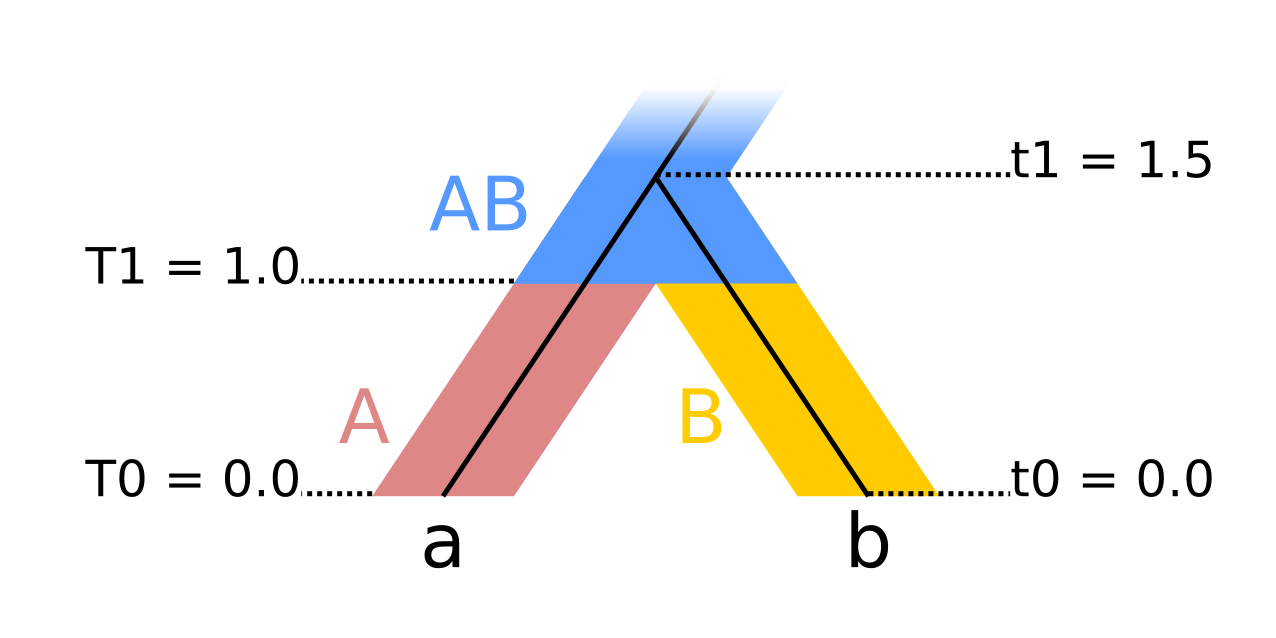
\includegraphics[width=70mm]{relaxed_clock.png}
\caption
{Two-species phylogeny used to illustrate species tree relaxed
clocks. There are two extant species ``A'' and ``B'', and one ancestral species ``AB''.
Within the species tree there is a single gene tree with extant individuals ``a''
and ``b''. The single speciation event occurs at time T1, and the single coalescence
event occurs at time t1. Gene tree rates are computed according to Table~\ref{tab:branchRateModel}}
\label{fig:branchRateModel}
\end{figure}

\begin{table*}[htb!]
\caption{Expected number of substitutions $\Sigma \mathbb{E}(S)$ for gene branches \textit{a, b} under a species tree relaxed clock}
\label{tab:branchRateModel}
\begin{threeparttable}
\begin{tabular*}{\textwidth}{@{\extracolsep{\fill}}cccccccccccc@{}}
\hline
Gene & Gene & \multicolumn{3}{c}{Length\tnote{2} $L$} & \multicolumn{3}{c}{Species rate\tnote{3} $R$} & \multicolumn{3}{c}{$\mathbb{E}(S) = c\cdot L\cdot R$} & \multirow{2}{*}{$\Sigma \mathbb{E}(S)$}\tabularnewline
branch & rate\tnote{1} $c$ & A & B & AB & A & B & AB & A & B & AB & \tabularnewline
\hline
a & \multirow{2}{*}{0.001} & 1.0 & 0.0 & 0.5 & \multirow{2}{*}{0.7} & \multirow{2}{*}{1.0} & \multirow{2}{*}{1.3} & 0.00070 & 0.00000 & 0.00065 & 0.00135\tabularnewline
b & & 0.0 & 1.0 & 0.5 & & & & 0.00000 & 0.00100 & 0.00065 & 0.00165\tabularnewline
\hline
\end{tabular*}
\begin{tablenotes}
\item[1] The overall substitution rate at a given locus.
\item[2] The length of a given gene tree branch within species tree branch A, B or AB.
\item[3] The substitution rate of species tree branch A, B or AB.
\end{tablenotes}
\end{threeparttable}
\end{table*}

The new species tree relaxed clock model is available in StarBEAST2. Branch
rate models that can be used with a species tree relaxed clock currently
include the well-established uncorrelated log-normal (UCLN) and uncorrelated
exponential (UCED) models \citep{10.1371/journal.pbio.0040088}, as well as the
newer random local clock model \citep{Drummond2010}. The current species tree
relaxed clock implementation estimates --- separately for each species tree
branch --- a single relative rate. However it is possible to imagine a further
relaxed model that estimates --- again separately for each species tree branch
--- hyperparameters for a prior distribution on substitution rates. This would
enable gene tree branch rates to be guided by the species tree, but still
allow some difference in response between genes.

\section{Results and Discussion}

\subsection{StarBEAST2 correctly implements the multispecies coalescent}

New methods must be shown to be correct implementations of the target model.
One way to accomplish this for MCMC methods is to estimate parameters from a
prior distribution using the MCMC kernel, and to also draw independent samples
from the same distribution by simulation. The resulting parameter
distributions should be identical if the implementation is correct. We used
this method to test the correctness of the novel features in StarBEAST2;
analytical population size integration, coordinated operators, and species
tree relaxed clocks. Simulated and StarBEAST2 distributions were identical for
species and gene tree topologies (Figure~S1,S2), species and gene tree node
heights (Figure~S3,S4), and for gene tree branch rates (Figure~S5,S6). This
combination of results supports the correctness of the StarBEAST2
implementation.

\subsection{Species tree relaxed clocks prevent SPILS}

When using concatenation to infer a species tree, SPILS causes apparent
substitution rate variation among predictable species tree branches. However
in an ultrametric (time tree) framework like BEAST, branch lengths are
constrained so that terminal species begin at time zero. We hypothesised that
if a relaxed clock is used with concatenation in an ultrametric framework,
SPILS will be absorbed as faster substitution rates for lineages that would be
lengthened by SPILS in a non-ultrametric framework.

In an ultrametric framework with a strict clock and no external (e.g. fossil,
biogeographical or known clock rate) calibrations, the substitution rate of
each branch is set to 1. This ensures that 1 unit of time is equivalent to 1
expected substitution. Using a relaxed clock with no external calibrations the
substitution rate of each branch can vary, but the expectation of the mean
rate of all branches is 1, preserving the relationship of 1 unit of time = 1
expected substitution. Therefore when SPILS causes the rates of some branches
to be faster than 1, the rates of some other branches will be slower than 1 to
keep the expected mean constant.

We used BEAST concatenation and StarBEAST2 with a species tree relaxed clock
to infer the branch lengths and substitution rates of simulated species trees
with the topology ((((A,B),C),D),E), using sequence alignments simulated using
a strict clock. Gene tree discordance will increase the estimated length of A,
B and C branches for these species trees \citep{Mendes01072016}, and as
hypothesised substitution rates for A and B branches inferred using
concatenation were biased towards being faster than the true rate of 1
(Figure~\ref{fig:spilsRates}). Estimated substitution rates for the C branch
were more variable, and could be faster or slower than 1. Substitution rates
estimated for the D and E branches were biased towards being slower than 1,
presumably to balance the mean rate. Concatenation also overestimated the
lengths of tip branches, another known bias when using concatenation to infer
a species tree \citep{Ogilvie01052016}. No biases were observed for the branch
rates or lengths estimated using StarBEAST2 (Figure~\ref{fig:spilsRates}).

\begin{figure*}[htb!]
\centering
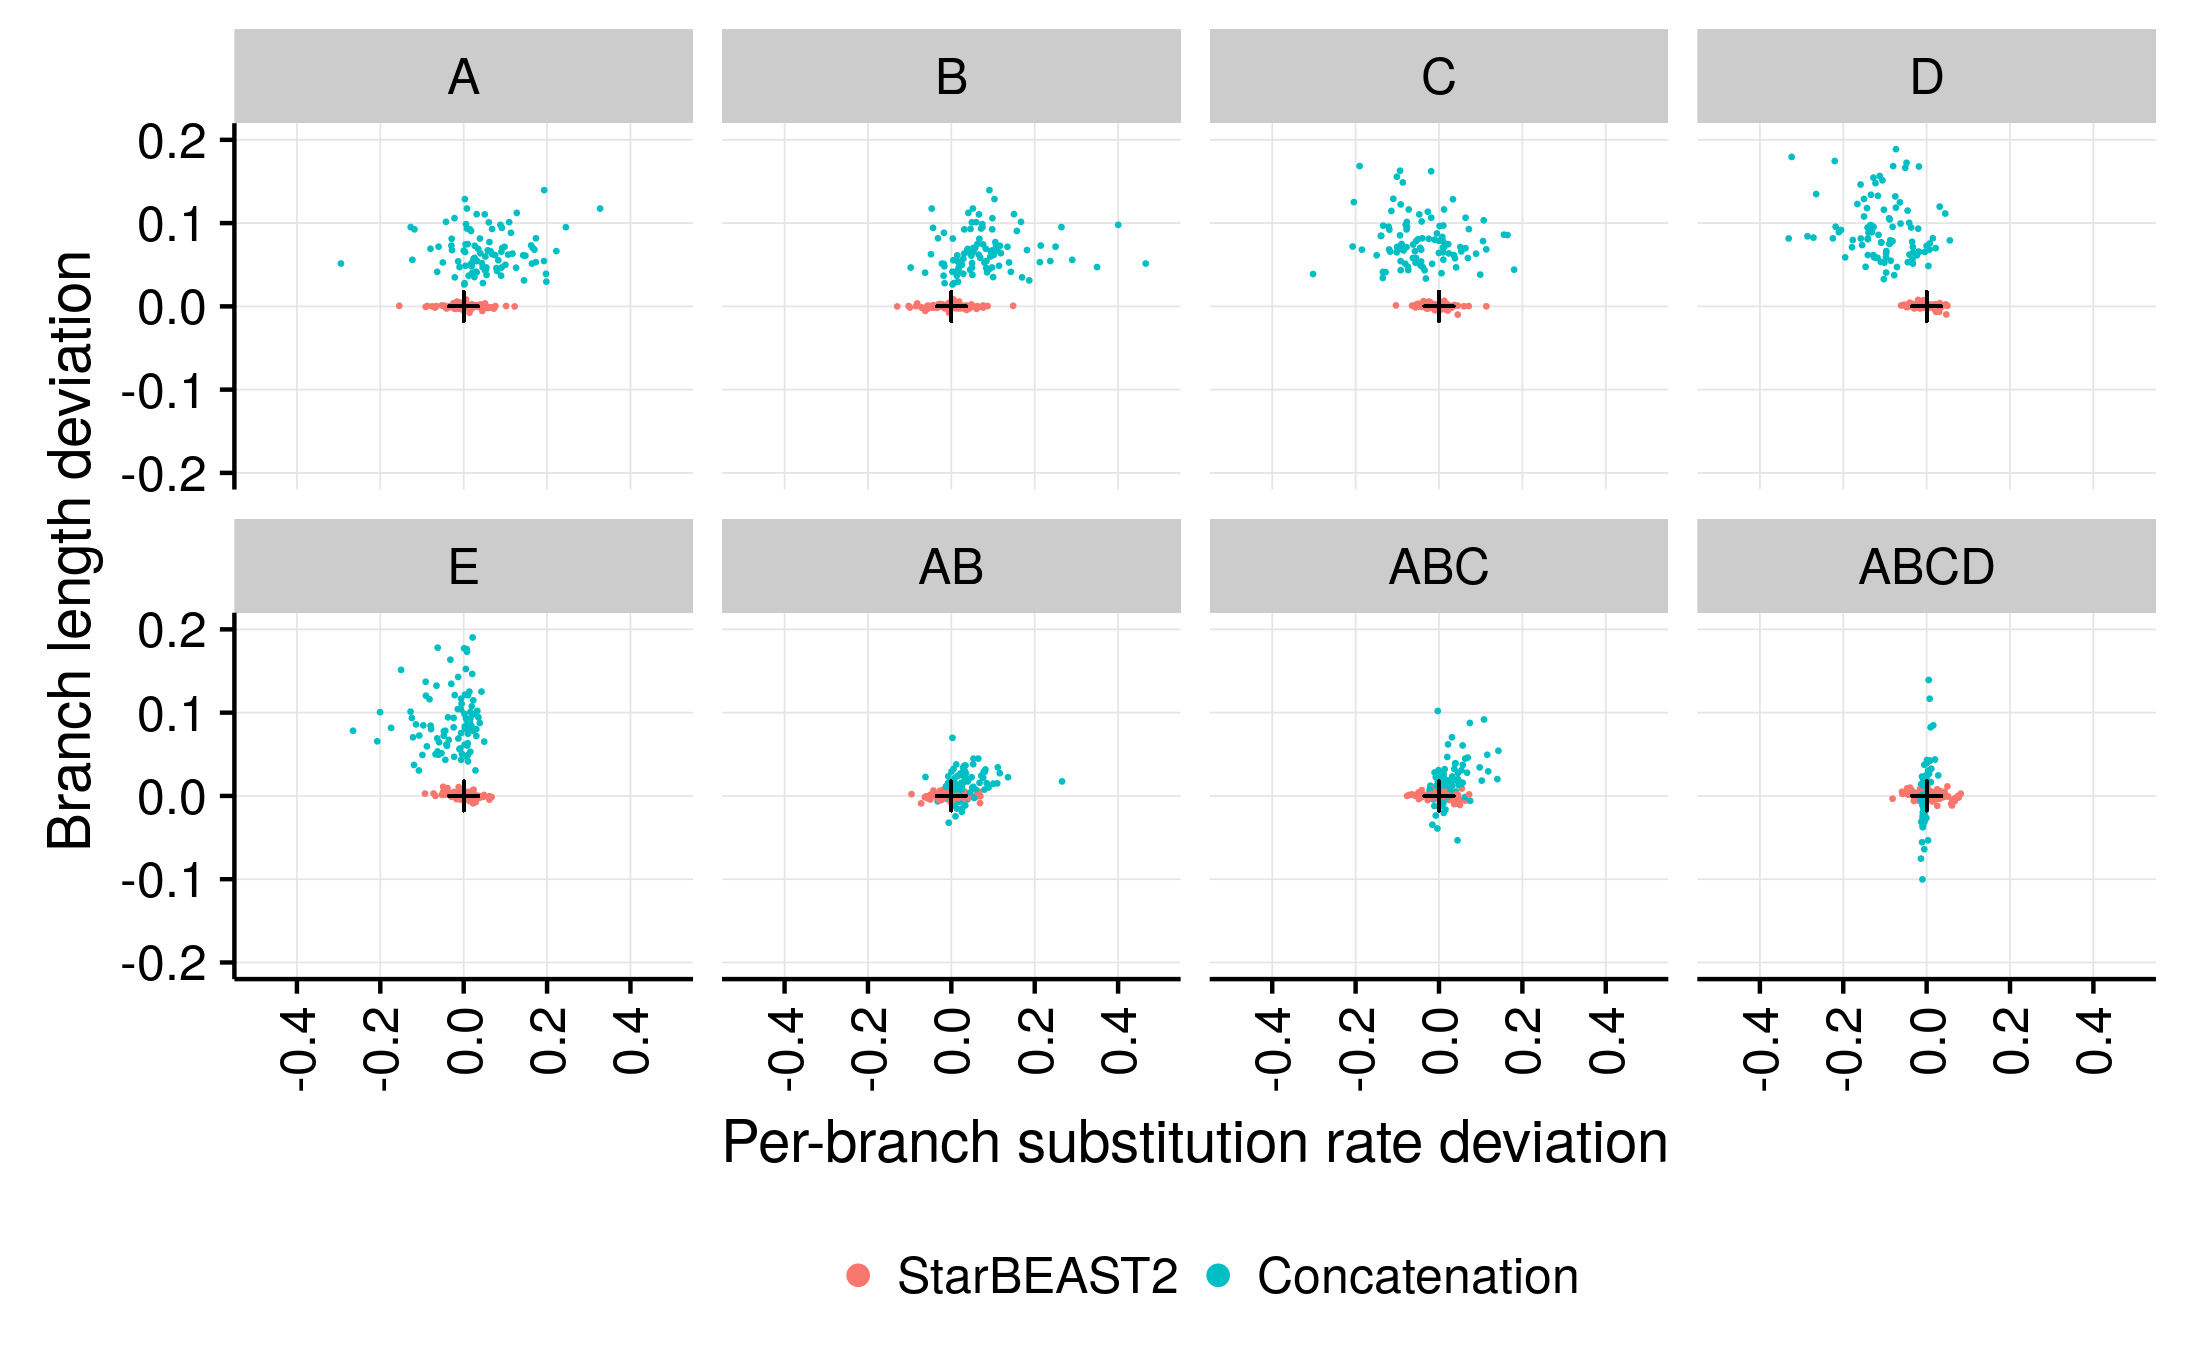
\includegraphics[width=130mm]{scatter.png}
\caption
{Accuracy of branch substitution rates and lengths inferred by BEAST
concatenation and StarBEAST2. Deviation is the difference of each estimated
rate and length from the true value. Estimated rates and lengths are the
posterior expectation of the overall substitution rate and length for each
species tree branch. Black crosses in each panel indicate the point of perfect
accuracy. Each panel shows the distributions for the labelled extant or
ancestral branch. N = 96.}
\label{fig:spilsRates}
\end{figure*}

A number of estimated branch rates had 95\% credible intervals that excluded
the true rate of 1 when using concatenation. If a study is testing whether
substitution rates vary across a species tree, those branch rates could be
erroneously interpreted as faster or slower than average. In our simulations,
the clock rate of the D branch would be inferred as slower than average in 37
out of 96 replicates (Figure~S7), despite the sequence data being simulated
using a strict clock. When applying the same 95\% credible intervals to branch
lengths, the true simulated length was excluded with just two exceptions for
all tip branches across all replicates using concatenation (Figure~S8). In
contrast, no erroneous results would be inferred for branch rates given the
same data using StarBEAST2, and out of the 768 total simulated non-root branch
lengths, only five erroneous results would be inferred (Figure~S7,S8).

\cite{Mendes01072016} demonstrated that SPILS causes systematic bias when
estimating branch lengths, and we show that this translates into systematic
bias when estimating per-branch substitution rates. Because the bias is caused
by incomplete lineage sorting which is a function of population sizes and
branch lengths, there is no reason to expect that large trees with varying
population sizes and branch lengths would be any less biased.

\subsection{Datasets used to characterise the new methodological approaches}

To characterise the performance of coordinated operators, methods of
population size integration and relaxed clocks, we tested StarBEAST2 using
empirical and simulated sequence data. The empirical data set used for this
analysis is from the North American chorus frog genus \textit{Pseudacris}, and
was originally collected and analysed by \cite{Barrow201478}. This data set
has sequences from 26 nuclear loci across 44 sampled individuals. The individuals
belong to 19 extant \textit{Pseudacris} lineages and two outgroup species.
\cite{Barrow201478} reported phased haplotypes but to avoid wasting
computational resources we used a single haplotype per individual.

A key metric of phylogenies that can be used to judge whether it is necessary
to employ MSC models is the average branch length in coalescent units
$\tau(2N_e)^{-1}$. In this study $N_e$ will always refer to the
effective population size of diploid individuals. Given short branch lengths,
likelihood-based or neighbour-joining concatenation is unable to infer accurate
species trees regardless of the number of loci used, but for long branch
lengths, concatenation is approximately as accurate as *BEAST
\citep{Ogilvie01052016}. Indeed concatenation can be considered a special
case of the MSC as the models converge when gene
trees are identical to the species tree \citep{NYAS:NYAS12747}. Using StarBEAST2, the average branch length within
this genus was estimated to be $2.81\tau(2N_e)^{-1}$. This is an
intermediate average length compared to the shallow simulations analysed by
\cite{Ogilvie01052016} which had a shorter average length of
$1.08\tau(2N_e)^{-1}$.

Each replicate of each \textit{Pseudacris} empirical analysis used the same
sequence data, and the true species tree topology, dates and rates were not
known with certainty. For performance results more generally applicable than a
single empirical system, and to measure the accuracy and coverage of
StarBEAST2 inference, we created a simulated data set of 30 replicates. A
unique species tree was simulated for each replicate, and gene trees and locus
sequences were simulated according to the MSC.

We simulated 26 nuclear loci from 21 extant species with two individual
haplotypes per species, very similar to the empirical data set size. The
simulation parameters, including the birth rate, death rate and population
sizes, were also chosen to be similar to estimated \textit{Pseudacris}
parameters. The simulated data set had an average branch length of
$2.99\tau(2N_e)^{-1}$, so the relative accuracy of MSC models compared
to concatenation should be comparable with empirical systems like
\textit{Pseudacris}.

\subsection{Coordinated height changing operators and analytical integration improve performance}

To determine which configuration of new features would achieve the best
performance, we ran StarBEAST2 using different combinations of operators,
methods of population size integration and clock models. To measure
convergence both effective sample size (ESS) per hour and ESS per million
states were computed for each independent chain. ESS per hour can be used to
calculate the total time required for a converged chain (nominally where ESS
equals or exceeds 200), and reflects how effectively operators explore the
space of trees and parameters, as well as the computational time required by
each operator proposal and likelihood calculation. In contrast, ESS per
million states reflects only the exploration of tree and parameter space
independently of calculation times. A variety of statistics were recorded for
each analysis (Table~S2-S7), and for each replicate the statistic with the
slowest ESS rate for that particular chain was used when computing the mean
and standard deviation of ESS per hour and per million states, and in the
rest of the paper.

Multiple linear regressions with log transformed ESS rates as the response
variables were used to measure the effect of coordinated topology changing
operators, coordinated node height changing operators, and the method of
population size integration. Each additional feature was treated as a binary
indicator variable so that we could quantify the relative performance as a
percentage by exponentiating the coefficient for each addition
(Table~\ref{tab:convergenceLM}).

\begin{table*}[htb!]
\caption{Relative performance of operators, population size integration and clock models.}
\label{tab:convergenceLM}
\begin{threeparttable}
\begin{tabular*}{\textwidth}{@{\extracolsep{\fill}}rlrrr@{}}
\hline
Clock model & ESS rate per & Topology\tnote{3} & Height\tnote{4} & Analytical\tnote{5}\tabularnewline
\hline
\multicolumn{5}{c}{\textit{Pseudacris} reanalysis}\tabularnewline
\hline
Strict & hour & 73\%{***} & 120\%{***} & 130\%{***}\tabularnewline
Strict & million states & 101\%\hphantom{***} & 129\%{***} & 143\%{***}\tabularnewline
GT-UCLN\tnote{1} & hour & 72\%{***} & 289\%{***} & 100\%\hphantom{***}\tabularnewline
GT-UCLN & million states & 100\%\hphantom{***} & 310\%{***} & 108\%\hphantom{***}\tabularnewline
ST-UCLN\tnote{2} & hour & 78\%{**}\hphantom{*} & 499\%{***} & 154\%{***}\tabularnewline
ST-UCLN & million states & 95\%\hphantom{***} & 484\%{***} & 163\%{***}\tabularnewline
\hline
\multicolumn{5}{c}{Simulated data}\tabularnewline
\hline
Strict & hour & 70\%{***} & 137\%{***} & 208\%{***}\tabularnewline
Strict & million states & 100\%\hphantom{***} & 148\%{***} & 225\%{***}\tabularnewline
GT-UCLN & hour & 68\%{***} & 231\%{***} & 228\%{***}\tabularnewline
GT-UCLN & million states & 98\%\hphantom{***} & 248\%{***} & 248\%{***}\tabularnewline
ST-UCLN & hour & 72\%{*}\hphantom{**} & 927\%{***} & 135\%{*}\hphantom{**}\tabularnewline
ST-UCLN & million states & 86\%\hphantom{***} & 907\%{***} & 144\%{**}\hphantom{*}\tabularnewline
\hline
\end{tabular*}
\begin{tablenotes}
\item[1] Gene Tree Uncorrelated Log-Normal relaxed clock
\item[2] Species Tree Uncorrelated Log-Normal relaxed clock
\item[3] Coordinated topology changing operators relative to na\"ive operators
\item[4] Addition of coordinated height changing operators
\item[5] Analytical integration of population sizes relative to MCMC integration
\item Values higher than 100\% indicate faster convergence, lower than 100\% indicate slower. {*}: $p < 0.05$, {**}: $p < 0.01$, {***}: $p < 0.001$. N = 30.
\end{tablenotes}
\end{threeparttable}
\end{table*}

Coordinated topology operators consistently and significantly reduced ESS
per hour, but had no significant effect on ESS per million states
(Table~\ref{tab:convergenceLM}), suggesting that coordinated topology
operators are no more effective than na\"ive operators at proposing new
states. A decrease in the number of states per hour (Figure~S9) shows that
they are more computationally expensive than na\"ive operators, and explains
the negative effect on ESS per hour.

\begin{figure*}[htb!]
\centering
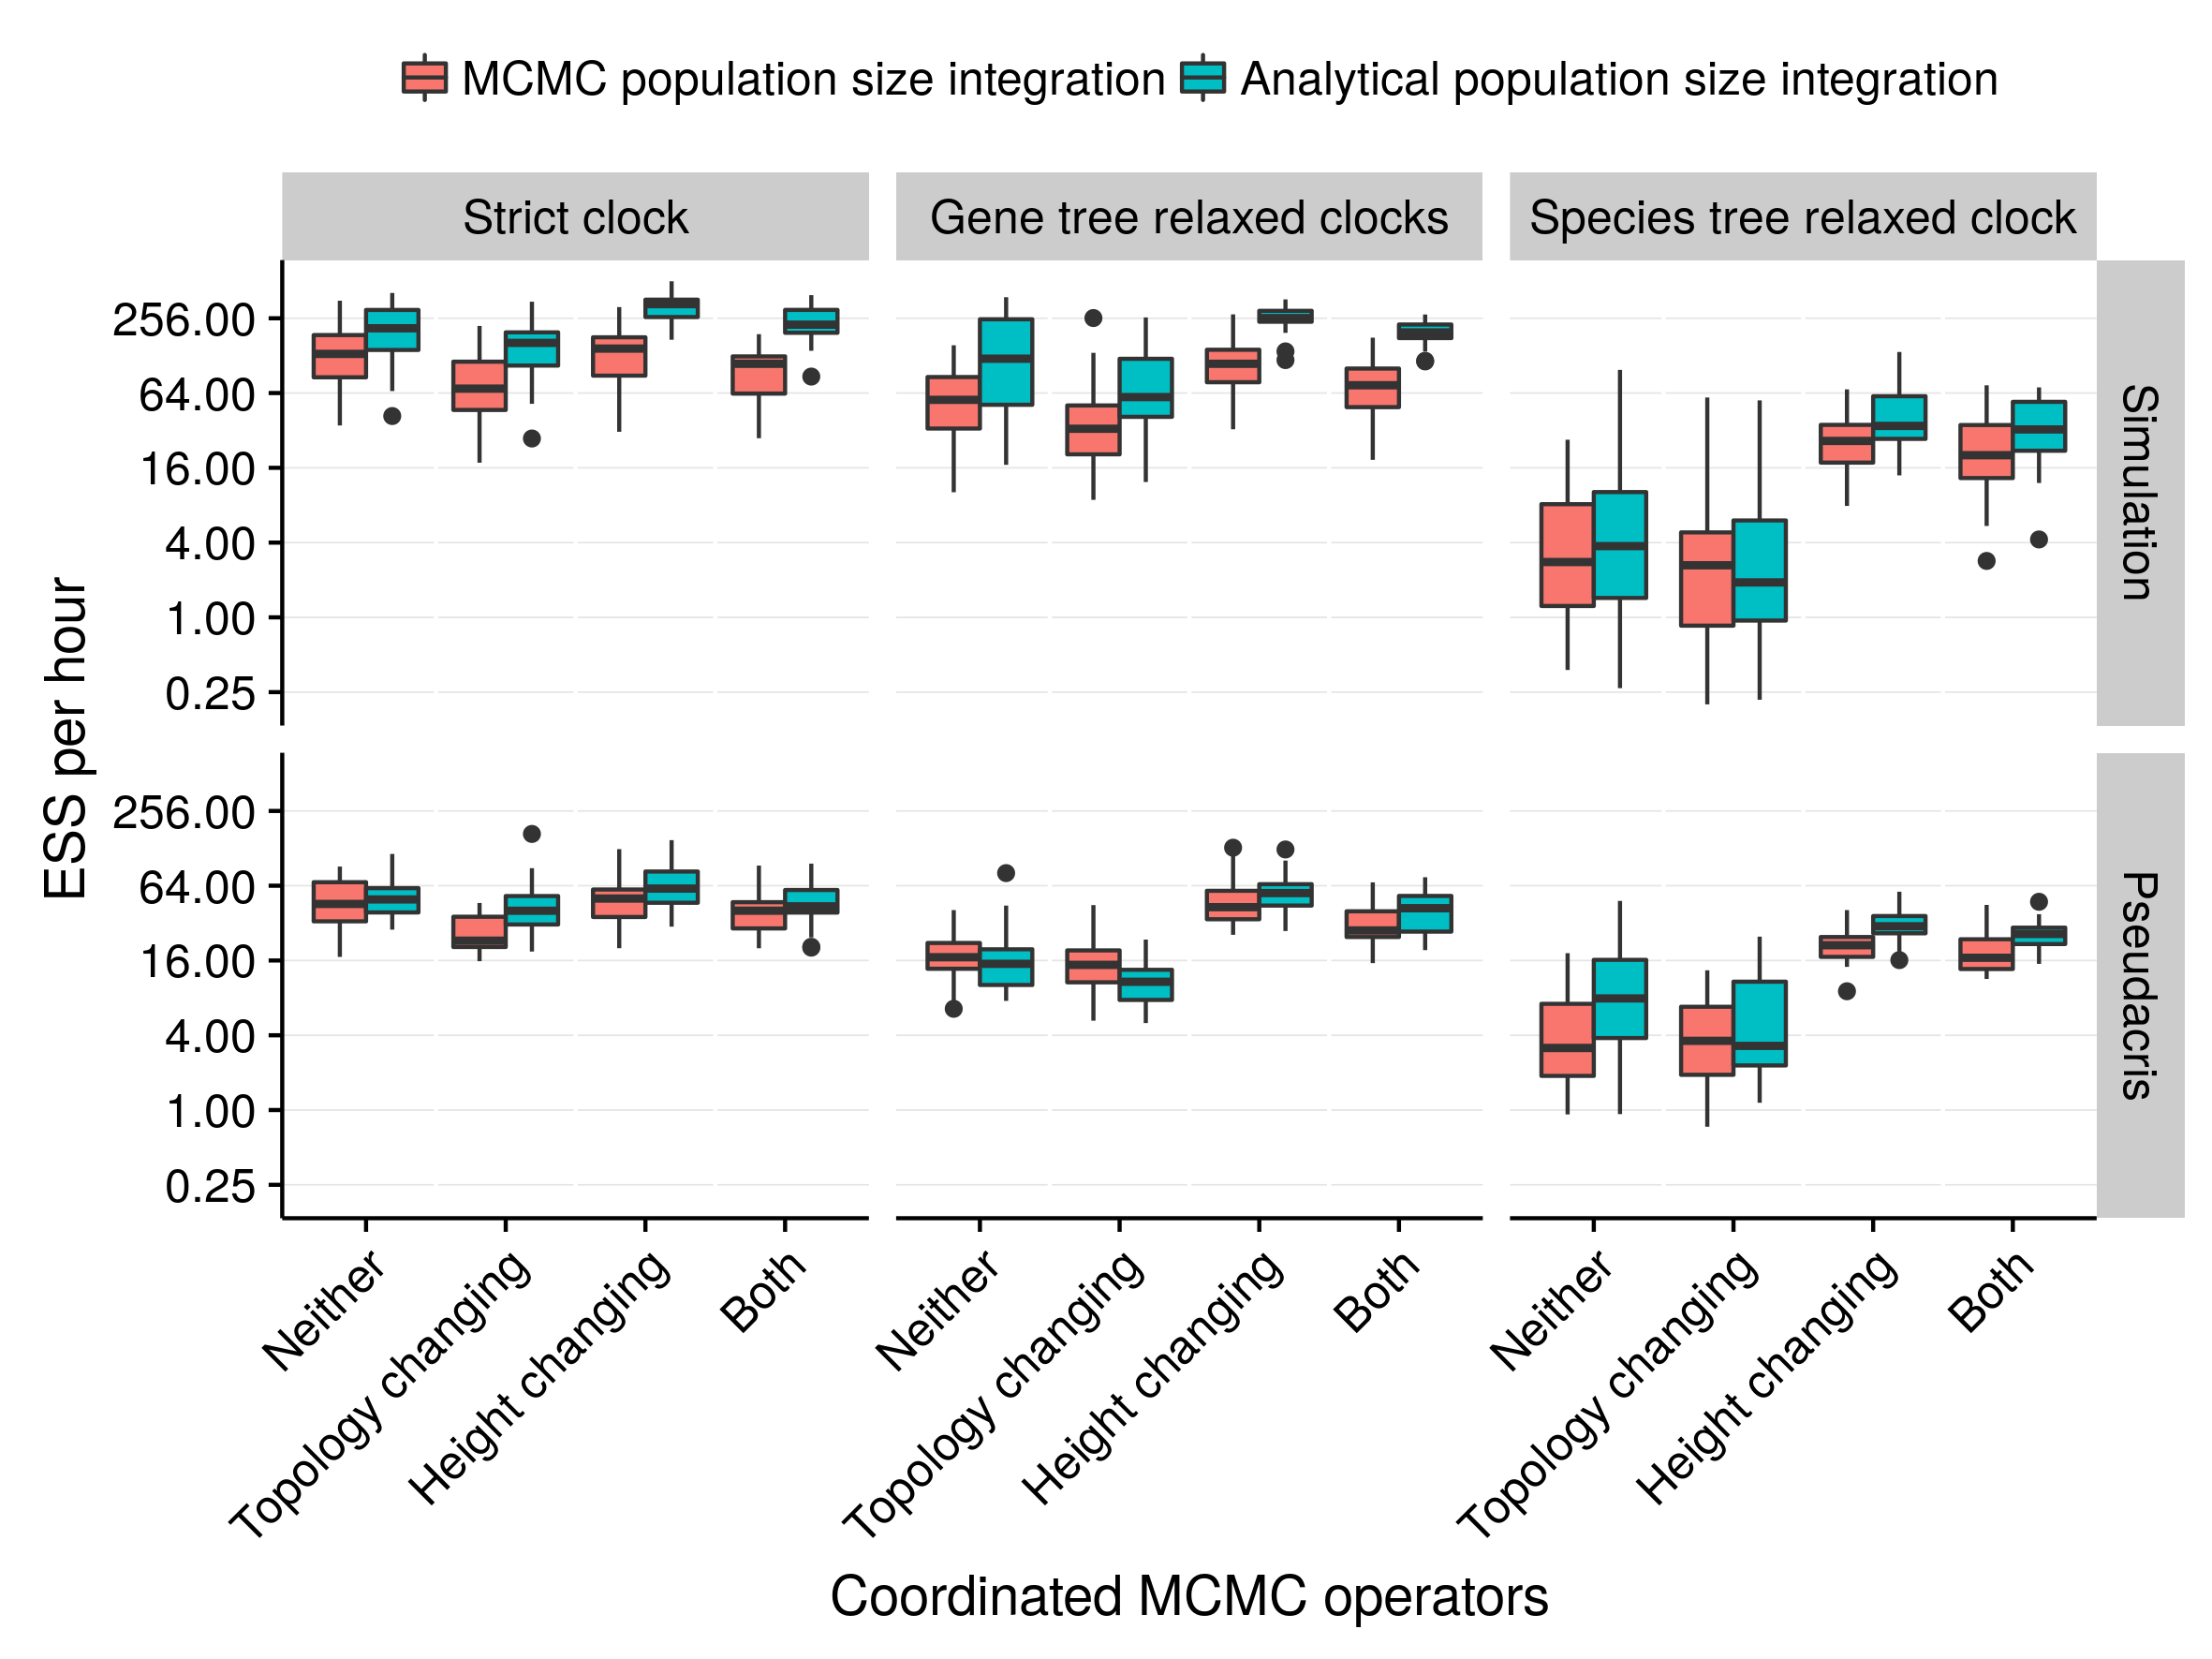
\includegraphics[width=130mm]{minimum-ess_per_hour-starbeast2.png}
\caption
{Impact of operators, population size integration and clock models on
convergence. The estimated sample size (ESS) per hour for a given replicate
used the smallest ESS out of all recorded statistics. Topology refers to the
replacement of na\"ive nearest-neighbour interchange and subtree prune and
regraft operators with coordinated operators. Height refers to the addition of
operators which make coordinated changes to node heights. Uncorrelated log-normal relaxed clocks were applied to either each gene tree (GT-UCLN) or to
the species tree (ST-UCLN). N = 30.}
\label{fig:realEssPerHour}
\end{figure*}

Coordinated height changing operators consistently and significantly
increased ESS per hour and ESS per million states, however the degree of
improvement depended on the clock model (Figure~\ref{fig:realEssPerHour}). For
strict clock analyses the increase in ESS per hour was modest at 1.2 times and
1.37 times for empirical and simulated data respectively, whereas for species
tree relaxed clocks the increase was 4.99 times and 9.27 times respectively
(Table~\ref{tab:convergenceLM}). The difference in species tree relaxed clock
performance suggests that coordinated height changing operators are necessary
for practical implementations of that model.

Analytical population size integration significantly improved ESS per hour
performance in all cases, with the exception of gene tree relaxed clocks
applied to the \textit{Pseudacris} data set. For the simulated analyses there
was a significant improvement to ESS per hour and ESS per million states
regardless of clock model (Table~\ref{tab:convergenceLM}).

Even with new operators and analytical population size integration, the ESS
per hour rates for species tree relaxed clocks were slower than for other
clock models (Figure~\ref{fig:realEssPerHour}). One reason is that changing a
species tree branch rate requires updating the phylogenetic likelihood for all
gene trees, so the computational cost is much higher than for strict or gene
tree relaxed clocks (Figure~S9).

\subsection{StarBEAST2 is an order of magnitude faster than *BEAST}

StarBEAST2 also optimises the core multispecies coalescent algorithms by
caching intermediate values and by using fast data structures. Operator
weights have also been refined by manual iteration for better performance.
Building on our results, by default StarBEAST2 enables coordinated height
changing operators and analytical population size integration, but keeps
na\"ive topology operators. To measure the combined improvement when
StarBEAST2 is applied to \textit{Pseudacris} data we compared the performance
of StarBEAST2 with default settings to *BEAST. For the simulation data set, we
compare StarBEAST2 with *BEAST and also with concatenation.

NGS data sets may have hundreds or thousands of loci. To gauge the performance
of StarBEAST2 applied to these data sets, we tested an empirical NGS data set;
ultraconserved element \citep[UCE;][]{Faircloth01102012} sequences from
Philippine shrews of the genus \textit{Crocidura} \citep{Giarla01092015}. This
data set consists of 1112 loci sampled from a total of 19 individuals, which
belong to 9 extant lineages. Again multiple statistics were recorded to
compute the ESS rate means and standard deviations.

Our simulation study confirmed that StarBEAST2 is many times faster than
*BEAST (Figure~\ref{fig:essPerHourComparison}). For simulated data the average
log convergence rate of StarBEAST2 with gene tree relaxed clocks was 5.54
$\ln(\nicefrac{ESS}{hour})$. This compares to 2.04 using *BEAST, an
increase in performance of $\exp(5.54 - 2.04) = 33.1$ times (Table~S2). In
fact, StarBEAST2 was
$\exp(4.18 - 2.04) = 8.5$ times faster at analysing 52 loci than *BEAST
was when analysing 26.

StarBEAST2 was an order of magnitude faster when analysing either
empirical data set. For gene tree relaxed clock reanalyses of
\textit{Pseudacris} the difference was $\exp(3.98 - 1.41) = 13.1$ times. For
50-locus \textit{Crocidura} reanalyses it was $\exp(2.79 - 0.11) = 13.8$ times
(Table~S4,S6).

The ESS per hour convergence of species tree relaxed clocks was lower than for
gene tree relaxed clocks. When applying StarBEAST2 to simulated data, gene tree relaxed clocks were
$\exp(5.54 - 3.71) = 6.2$ times faster than using species tree relaxed clocks (Table~S2). The difference was much smaller for empirical data;
for \textit{Pseudacris} reanalyses gene tree relaxed clocks were $\exp(3.98 -
3.44) = 1.7$ times faster, and for \textit{Crocidura} they were $\exp(2.79 -
2.12) = 2.0$ times faster (Table~S4,S6). In all three cases species tree relaxed clocks
using StarBEAST2 were still faster than gene tree relaxed clocks using *BEAST
(Figure~\ref{fig:essPerHourComparison}).

\begin{figure*}[htb!]
\centering
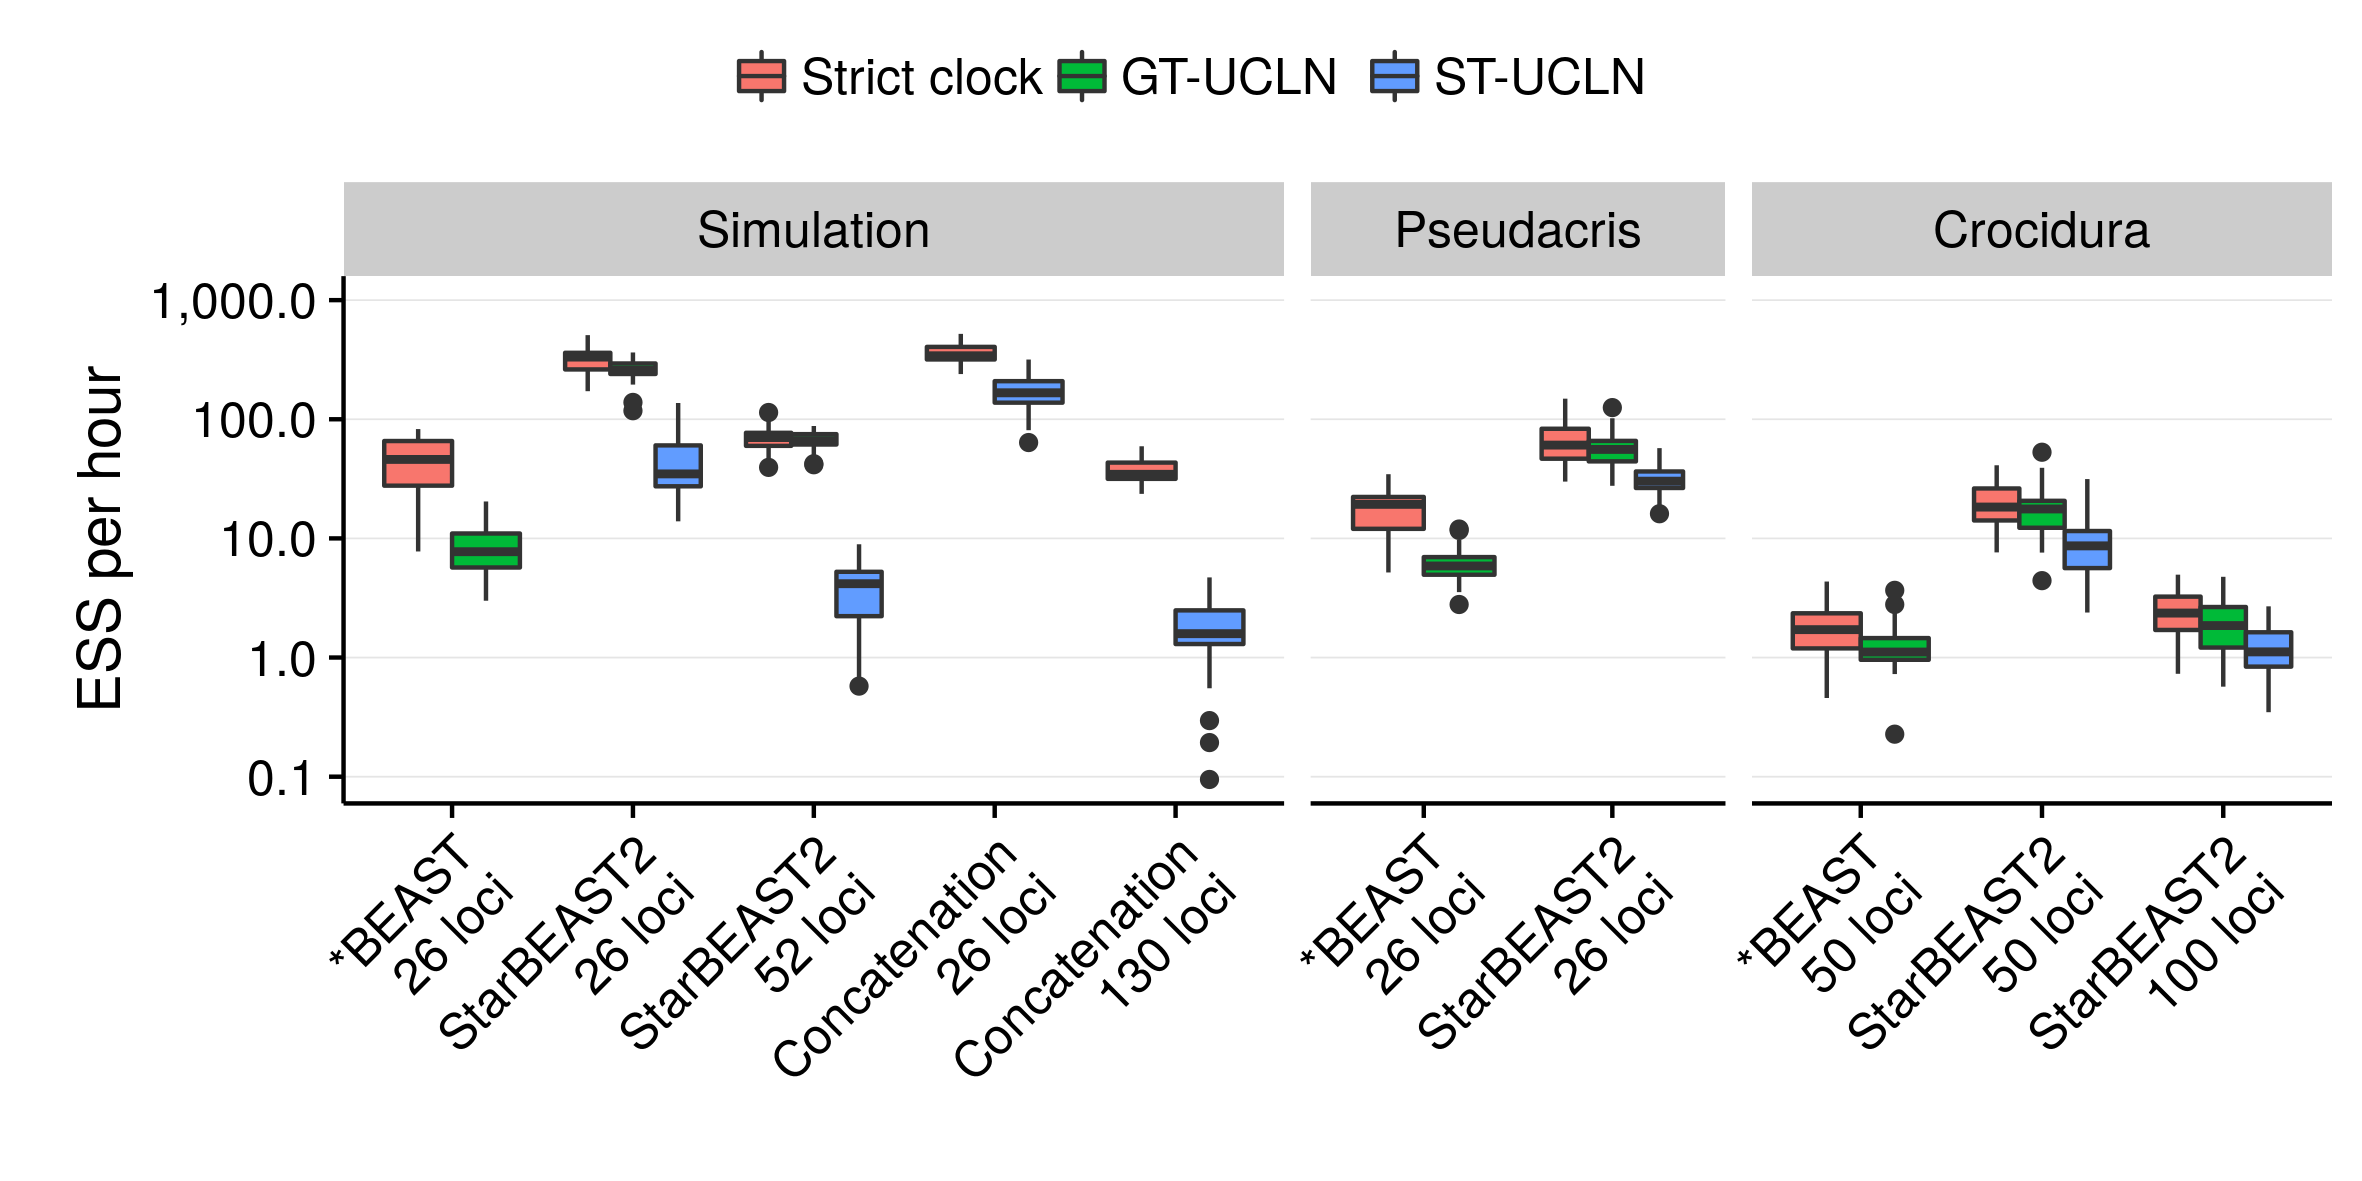
\includegraphics[width=130mm]{minimum-ess_per_hour-comparison.png}
\caption
{Convergence of different methods applied to simulated and empirical data
sets. The estimated sample size (ESS) per hour for a given replicate used the
slowest ESS rate out of all recorded statistics. Methods are BEAST
concatenation, *BEAST, and StarBEAST2 with uncorrelated log-normal relaxed
clocks applied to the gene trees (GT-UCLN) or to the species tree (ST-UCLN).
Two \textit{Pseudacris} *BEAST outliers with ESS rates below 0.1
are not shown.  N = 30.}
\label{fig:essPerHourComparison}
\end{figure*}

The increased performance of StarBEAST2 will enable researchers to analyse
sequence data more quickly and disseminate their findings sooner; a large MCMC
analysis which would currently take three months may now be performed in one
week. In the case of phylogenomic data which has been subsetted for use with
*BEAST, StarBEAST2 can be used to analyse more data for more
precise estimates of species trees and other parameters in the same amount of
time as a more limited *BEAST analysis.

\subsection{Species tree branch length accuracy and coverage}

Bayesian methods like StarBEAST2 produce both point estimates and credible
intervals of inferred parameters. Ideally the point estimates will be
accurate, and the credible intervals will include the corresponding true
values. Point estimates made by *BEAST and StarBEAST2 of both tip and internal
branch lengths were more accurate than those made by concatenation
(Figure~\ref{fig:branchLengthsError}A,B).

The inaccuracy of tip branch lengths inferred using concatenation was driven
by a strong bias towards overestimating branch lengths. For some replicates
the sum of estimated tip branch lengths was more than double the sum of
simulated tip branches lengths (Figure~\ref{fig:branchLengthsError}C).
Relatively little overestimation of internal branch lengths was observed when
using concatenation (Figure~\ref{fig:branchLengthsError}D).

Biased tip branch lengths are important because many published phylogenies show
evidence of a slowdown in diversification rate \citep{Moen2014190}. If the
ages of extant species are overestimated, this will artificially reduce the
number of recent speciation events, mimicking a slowdown. We suggest that
accurate inference of changing diversification rates requires species trees
inferred by fully Bayesian MSC methods like StarBEAST2.

Using a species tree relaxed clock with StarBEAST2 improved the coverage of branch
length credible intervals (Figure~\ref{fig:branchLengthsError}E,F), but even
when using a strict clock most simulated tip and internal branch lengths were
within the corresponding credible intervals. This suggests that a strict clock
model may be sufficient for studies using StarBEAST2 where substitution rate
variation is not of direct interest. When using a strict clock with
concatenation most internal branch lengths were outside the credible interval,
but when using a relaxed clock were usually within the credible interval
(Figure~\ref{fig:branchLengthsError}E). However even when using a relaxed
clock, tip branch lengths were usually outside the credible intervals inferred
by concatenation (Figure~\ref{fig:branchLengthsError}F).

\begin{figure}[htb!]
\centering
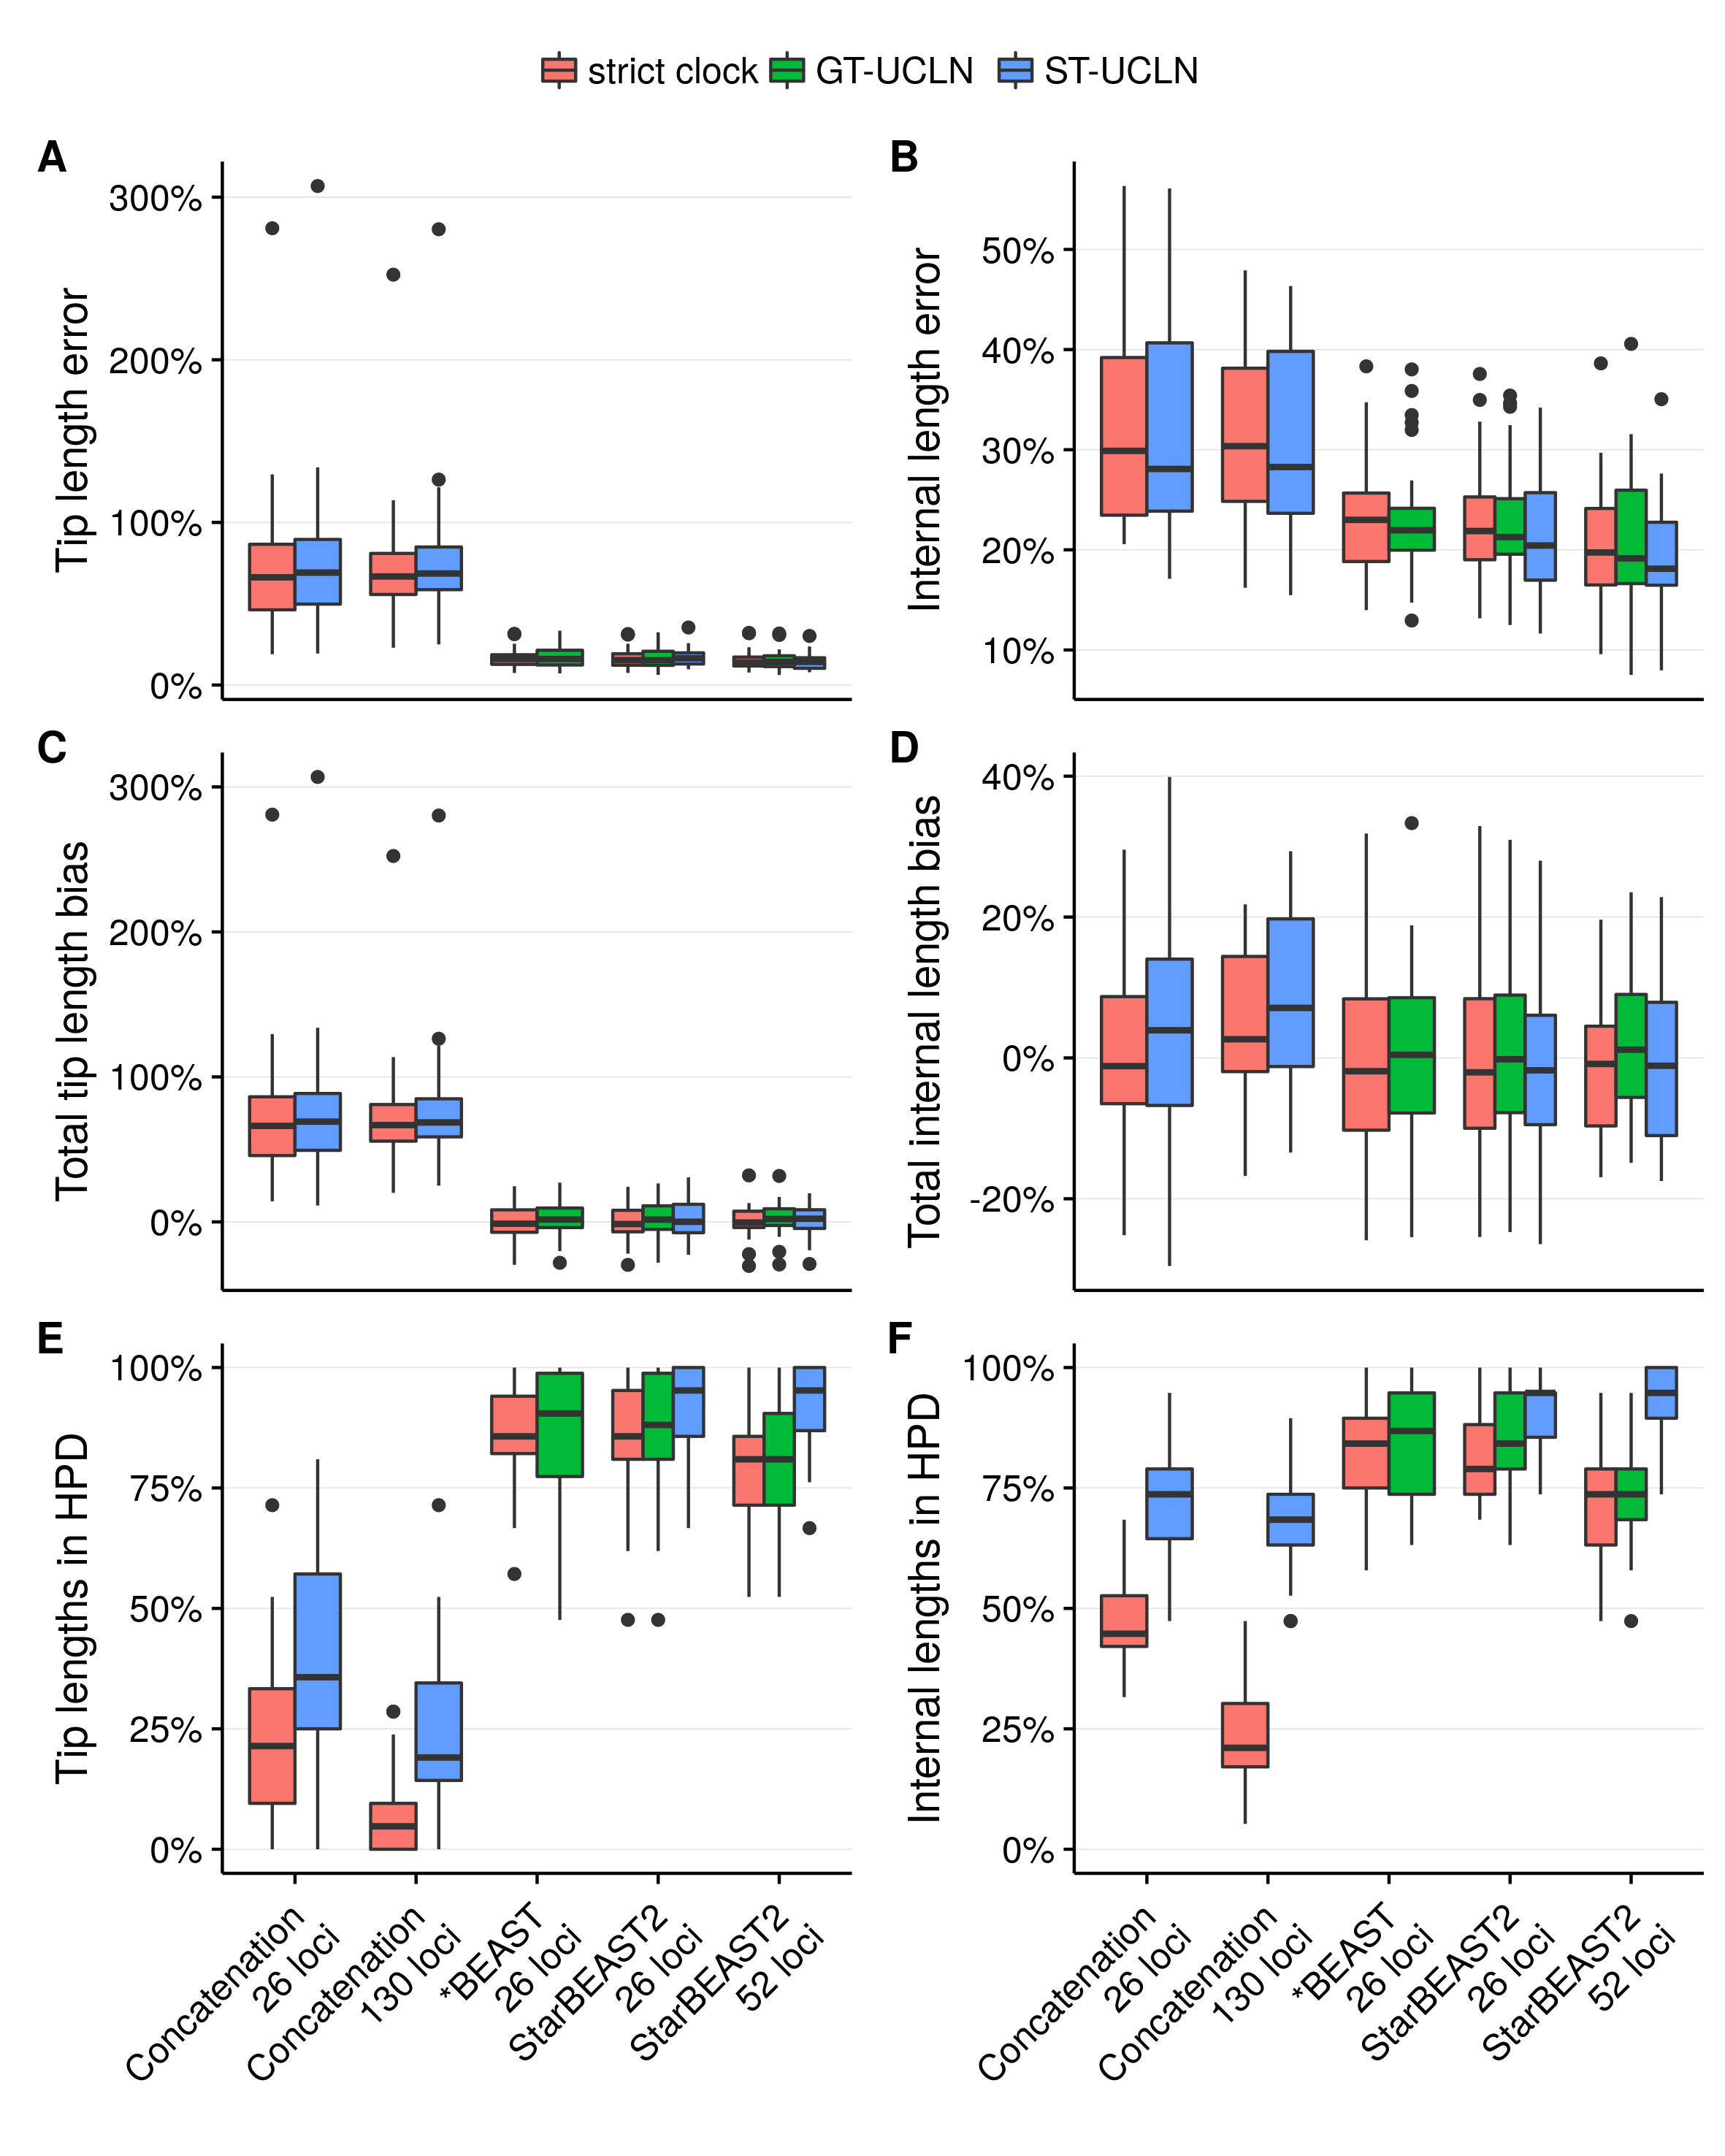
\includegraphics[width=130mm]{branch_length_accuracy_phased.png}
\caption
{Accuracy and coverage of species branch lengths using different methods. Methods are StarBEAST2,
*BEAST and BEAST concatenation with uncorrelated log-normal relaxed clocks applied
to the gene tree (GT-UCLN) or to the species tree (ST-UCLN). (A,B) The sum of absolute
differences between estimated and simulated branch lengths as a percentage of true
tree length. (C,D) The difference between the sum of estimated branch lengths and the
sum of true branch lengths as a percentage of the sum of true branch lengths. (E,F) The
percentage of true branch lengths present within the corresponding 95\% highest posterior density (HPD)
credible intervals. N = 30.}
\label{fig:branchLengthsError}
\end{figure}

Using unphased sequences with ambiguity codes for heterozygous sites improved
the accuracy of concatenation by reducing the bias in tip lengths to less than
40\% (Figure~S10). Topological accuracy was not improved by using unphased
sequences (Figure~S11). Ambiguity codes are treated by most
phylogenetic methods (including BEAST) as base call uncertainty,
indicating the nucleotide at a given site could be one of several
possibilities. When used with unphased sequences, they actually indicate the
presence of two nucleotides simultaneously, which is therefore a model violation.
Using concatenation to analyse unlinked loci is also a model violation, but in
the region of parameter space investigated by this simulation study the two
errors may \textit{partially} cancel out.

\subsection{Species tree topology accuracy and coverage}

We used the rooted Robinson-Foulds distance metric to measure the accuracy of
maximum clade credibility (MCC) point estimates of species tree topologies. By
this metric concatenation using 130 loci was similar in accuracy to StarBEAST2
using 26 loci (Figure~\ref{fig:treeTopologyError}A). Using species tree
relaxed clocks with StarBEAST2 was slightly more accurate than using strict
clocks, but relaxed clocks did not improve the accuracy of concatenation
(Figure~\ref{fig:treeTopologyError}A).

As with branch lengths, using a relaxed clock with concatenation or a species
tree relaxed clock with StarBEAST2 improved coverage. Regardless of clock
model the coverage of concatenation was low; in less than 50\% of replicates
was the simulated topology in the credible set
(Figure~\ref{fig:treeTopologyError}B).

\begin{figure}[htb!]
\centering
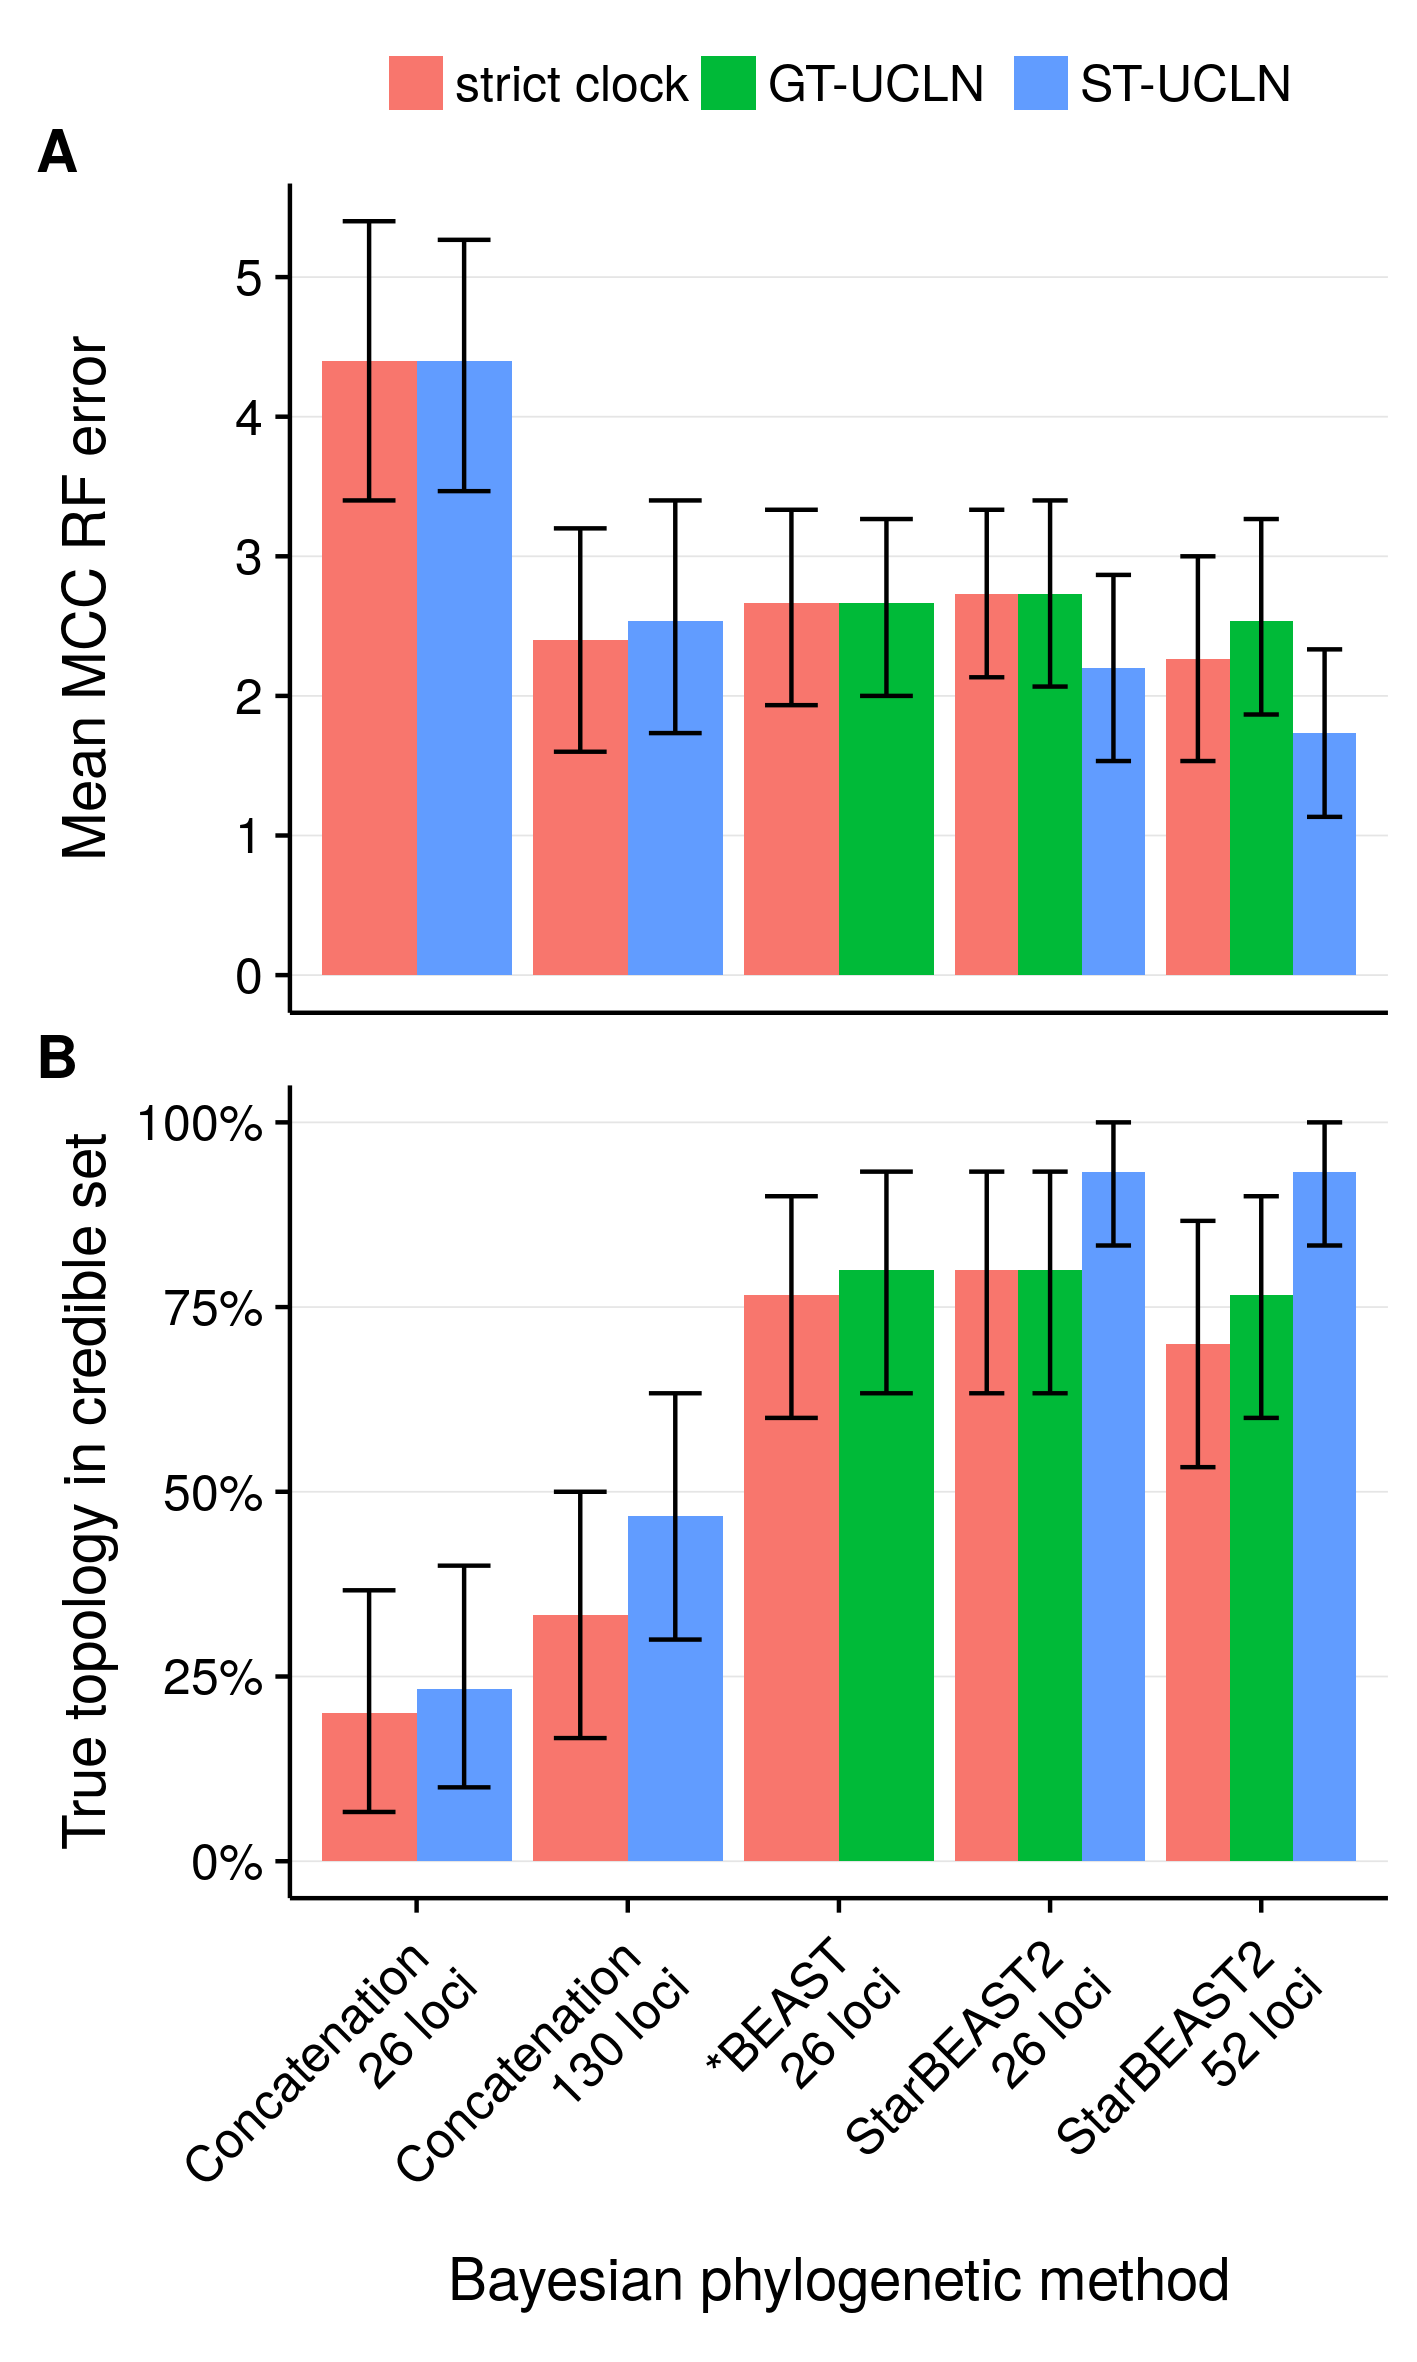
\includegraphics[width=70mm]{topology_accuracy_phased.png}
\caption
{Accuracy and coverage of species tree topologies using different methods.
Methods are StarBEAST2, *BEAST and BEAST concatenation with uncorrelated
log-normal relaxed clocks applied to the gene tree (GT-UCLN) or to the species
tree (ST-UCLN). (A) The average rooted Robinson-Foulds (RF) distance between the
maximum clade credibility (MCC) species tree topology and the
simulated true topology. (B) The percentage of true species tree topologies
within the 95\% credible set of topologies. Error bars are 95\% confidence
intervals calculated by bootstrapping. N = 30.}
\label{fig:treeTopologyError}
\end{figure}

\subsection{StarBEAST2 is superior at inferring substitution rates}

While the convergence of species tree relaxed clock analyses took longer than
for gene tree relaxed clocks in StarBEAST2, species tree relaxed clocks enable
inference of species branch rates within an MSC framework. To gauge the
accuracy of estimated branch rates, we used simple linear regressions with the
true rate of each simulated branch as the explanatory variable, and the
posterior expectation of the rate of that branch (conditional on the
corresponding clade being monophyletic in the posterior samples) as the
response variable. If all estimates are equally proportional to the truth,
then the $R^2$ coefficient of determination will equal 1. There are intrinsic
limits to our ability to estimate substitution rates, primarily that branch
length is confounded with substitution rate \citep{Thorne01092002}.

For analyses of simulated data using 26 loci the $R^2$ using StarBEAST2 was
$0.39$ and by doubling the number of loci to 52 was increased to $0.43$. In
contrast the $R^2$ when using concatenation with 26 loci was $0.26$ and even after
increasing the number of loci to 130 it was only $0.33$, in either case worse
than StarBEAST2 using 26 loci (Figure~\ref{fig:branchRates}). StarBEAST2 is
clearly superior to concatenation at inferring branch rates.

Concatenation is an even worse estimator of branch rates when using unphased
sequences with ambiguity codes for heterozygous sites. When applying
concatenation to either 26 or 130 loci, $R^2$ was very weak at $0.12$ regardless
of the number of loci (Figure~S12).

\begin{figure}[htb!]
\centering
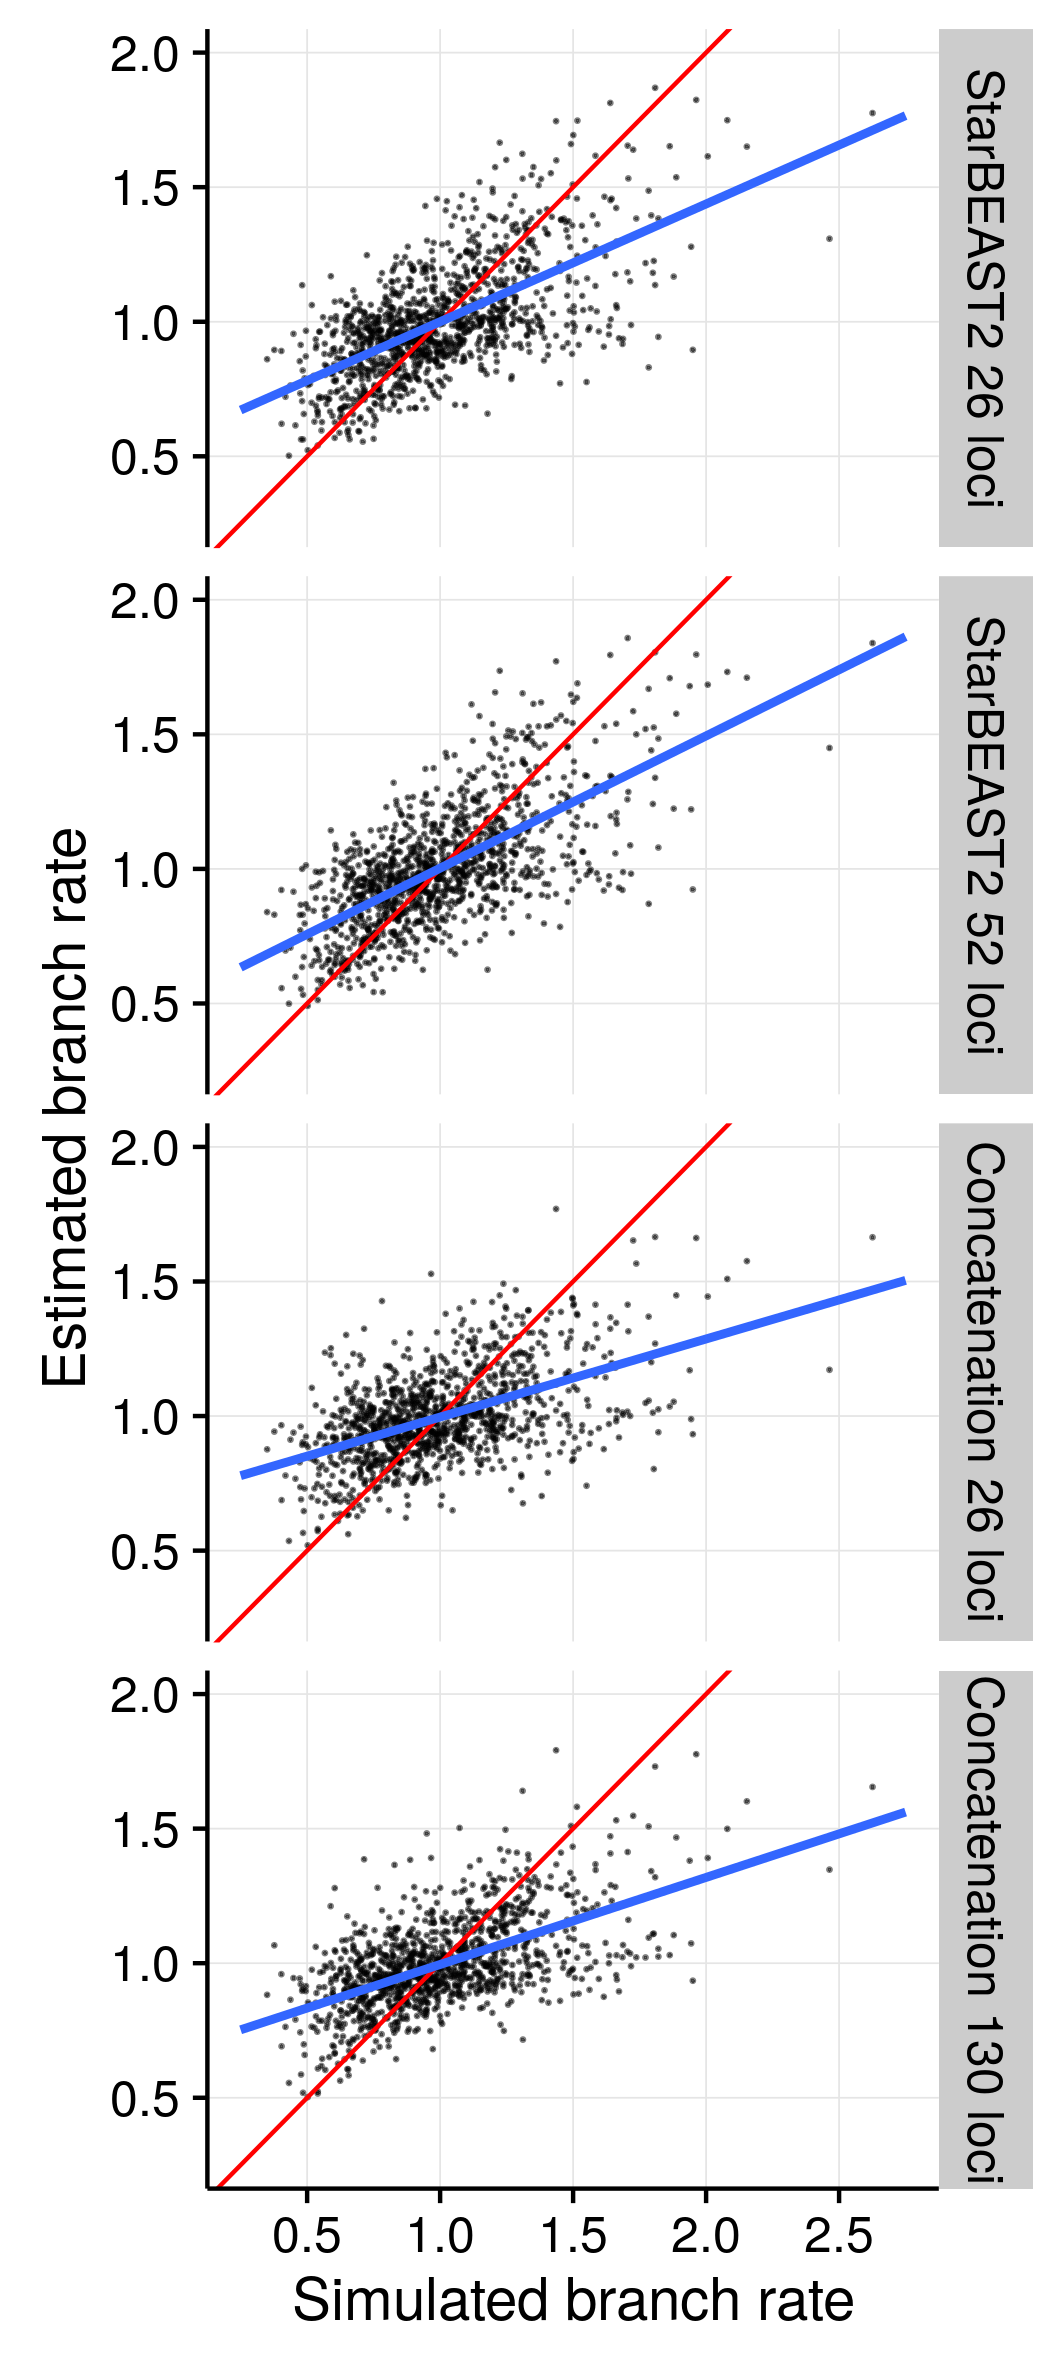
\includegraphics[width=70mm]{branch_rates_phased.png}
\caption
{Estimates of species tree branch rates using BEAST concatenation versus
StarBEAST2. Estimated rates are the posterior expectations of each branch rate
from each replicate. Root branch rates, which were fixed at 1, were excluded.
In blue are simple linear regression lines of best fit, and in red are the $y
= x$ lines showing a perfect relationship between estimates and truth. N = 30.}
\label{fig:branchRates}
\end{figure}

\section{Conclusions}

When estimating divergence dates and substitution rates, the choice is often
between using a subset of available loci with a fully Bayesian MSC method, or
all available loci with concatenation. Researchers have often opted for the
second choice, but we have shown that concatenation may not accurately
estimate the ages of extant species or per-species substitution rates, even
for trees of intermediate branch lengths. The increased performance of
StarBEAST2 should further encourage the adoption of fully Bayesian MSC methods
for estimating divergence times, and the new species tree relaxed clock will
enable accurate inference of species branch rates despite ILS. StarBEAST2 is
free and open source software; source code, development history and multiple
tutorials are available on GitHub (\url{https://github.com/genomescale/starbeast2}).

\section{Materials and Methods}

For all StarBEAST2, *BEAST and concatenation analyses, the version of BEAST
used was 2.4.4. For all simulations, the version of biopy \citep{biopy} used
was 0.1.9.

\subsection{Mathematical correctness of StarBEAST2}

Simulated trees were generated using biopy, and trees sampled from a prior
distribution were generated using StarBEAST2 with all new features enabled.
This included analytical integration of population sizes, coordinated tree
topology and node height changing operators, and a species tree relaxed clock.
100,000 species trees were simulated, one gene tree was simulated per species
tree with a rate of 0.5, and a second gene tree was simulated per species tree
with a rate of 2.0.

100,000 species trees, 100,000 half rate gene trees and 100,000 double rate
gene trees were sampled from the prior at a rate of one every 1000 after a
10\% burn-in period.

Identical parameters were used for the simulation and for the StarBEAST2 run
including the prior distributions. We fixed the number of species at 5 and the
number of haplotypes per species at 1. The birth and death rates were fixed at
200 and 100 per substitution respectively. Haploid population sizes followed
an inverse gamma distribution with shape $\alpha = 3$ and scale $\beta =
0.004$.

This procedure was repeated for both UCLN and for UCED species branch rates.
Branch rates were sampled from a lognormal or exponential distribution, in
either case with a mean of 1, discretised into 100 bins.

\subsection{Reanalysis of \textit{Pseudacris} sequence data}

Phased and aligned \textit{Pseudacris} sequence data were retrieved from Dryad
(\url{http://dx.doi.org/10.5061/dryad.23rc0}). Replicating the original
analysis we applied the HKY nucleotide substitution model \citep{Hasegawa1985}
to 22 out of 26 nuclear loci and the GTR model \citep{Tavare1986} to the
remaining 4. For all models we used four discrete $\Gamma$ categories to
accommodate among-site rate variation \citep{Yang1994}. Transition/transversion
rates and ratios and rate variation shape parameters were estimated, and
empirical base frequencies used, all separately for each locus. The relative
substitution rate of each locus was estimated using a lognormal prior with a
mean $\mu$ in real space of 1 and a standard deviation $\sigma$ of 0.6. We
used a single haplotype sequence per individual per locus, halving the total
number of sampled sequences to avoid wasting computational resources.

For inference of \textit{Pseudacris} trees, we ran 30 independent StarBEAST2
chains for all 24 conditions for a total of 720 chains. The conditions were
each possible combination of strict, species tree relaxed or gene tree relaxed
clocks, analytical or MCMC population size integration, coordinated or na\"ive
topology changing operators, and the inclusion or exclusion of coordinated
height changing operators. Each chain used the same sequence data but was a
partially independent estimate of convergence because a different random seed
was used to initialise each chain.

A birth-death prior was used for the species tree and both the net
diversification and extinction fraction hyperparameters were estimated. A
gamma prior was used for MCMC estimated population sizes with a shape fixed at
2 and an estimated mean population size hyperparameter, matching the original
*BEAST model \citep{Heled01032010}. The number of branch rate categories was
equal to the number of estimated branch rates (as is the default in BEAST 2),
and the standard deviation of the UCLN clock model was fixed at 0.3.

To ensure convergence of all chains, we ran each chain for an initial length
of $2^{24} =$ 16,777,216 states, sampling every $2^{11} =$ 2,048 states. Initial
chain lengths and sampling rates for all other analyses are in Table~S8. ESS
values were computed for all recorded statistics after discarding 12.5\% of
state samples as burn-in. Recorded statistics included (1) the posterior
probability, (2) the coalescent probabilities of gene trees, (3) the overall
prior probability, (4) the birth death prior probability of the species tree,
(5) the phylogenetic likelihood, (6) the net diversification rate, (7) the
extinction fraction, (8) the mean population size, and (9) the height of the
species tree.

If any recorded statistic had an ESS below 200, the chain was resumed until
the length of the chain had doubled. ESS values were then re-evaluated, again
after discarding 12.5\% of state samples. The length of a chain was
continually doubled and ESS values re-evaluated until the ESS values of all
recorded statistics were above 200. The rate at which trees and statistics
were sampled was halved with every chain doubling so that the total number of
samples remained constant. Two *BEAST GT-UCLN chains still had insufficient
ESS values after running for $2^{34} =$ 17,179,869,184 states, but all other
chains had converged. Estimated ESS values for all chains were used for
analyses of computational performance.

ESS per hour was calculated by dividing the final ESS value for a given
statistic by 87.5\% of the total CPU time used by that chain to account for
burn-in. Likewise ESS per million states was calculated by dividing the final
ESS value by 87.5\% of the total number of the states in the chain, then
multiplied by one million. For all analyses of computational performance
including graphs and linear models, the ESS rate for any given chain was that
of the slowest converging statistic for that particular chain.

Average branch length in coalescent units was calculated by concatenating the
output (after discarding the first 12.5\% of states as burn-in from each
chain) of all 30 chains which used the combination of MCMC population size
integration, na\"ive topology operators, coordinated node height operators and
species tree branch rates. For every sample in the combined posterior
distribution, the coalescent length of each branch $\tau(2N_e)^{-1}$ was
calculated from its length in substitution units $\tau$ and its effective
population size $N_e$. The mean coalescent length of all branches across all
samples was taken as the average.

\subsection{Testing the effects of SPILS on estimated substitution rates}

To test how SPILS affected estimates of per-species branch substitution rates,
96 fully asymmetric species trees were simulated with the topology
((((A,B),C),D),E). All species trees were simulated according to a pure birth Yule
process \citep{Yule21} with a speciation rate of 10 per substitution.

Haploid population sizes for each branch were chosen independently from an
inverse gamma distribution with a shape of 3 and a scale of 0.2. 100 gene trees
with one individual per extant species were then simulated for each species tree
according to the MSC process using biopy. Finally 1000nt sequence alignments
were then simulated for each gene tree according to the Jukes-Cantor
substitution model \citep{JUKES196921}, equal base frequencies, no among-site
rate variation, a strict molecular clock, and a substitution rate of 1 for each
locus. Sequence alignments were simulated using Seq-Gen \citep{Rambaut01061997}.

BEAST concatenation and StarBEAST2 were then used to estimate the branch rates
and divergence times with the species tree topology fixed to the truth. The same
substitution model used for simulating sequences (i.e. Jukes-Cantor, no rate
variation among sites or loci) was also used for inference. UCLN relaxed
clocks were applied to the tree inferred by concatenation and to the
StarBEAST2 species tree.

The same strategy as applied to \textit{Pseudacris} was used to ensure
convergence of StarBEAST2, but for concatenation mean population sizes and coalescent
probabilities are not part of the model and so were not recorded.

For every converged chain, the posterior expectation and 95\% credibility
intervals of per-species branch rates were calculated using the TreeAnnotator
program supplied with BEAST.

\subsection{Simulations to measure computational and statistical performance}

All simulation parameters were chosen to be broadly similar to those observed in
or estimated from the \textit{Pseudacris} data set.

First, 30 species trees were simulated according to a birth-death process
\citep{Gernhard2008769} using biopy with 21 extant species, a speciation rate
of 100 and a death rate of 30. This corresponds to a net diversification rate
of 70 and an extinction fraction of 0.3. Haploid population sizes for each
branch were chosen independently from a gamma distribution with a shape of 2
and a scale of 0.002. For a species with annual generation times, as is the
case for at least some \textit{Pseudacris} species \citep{10.2307/1446044},
and a substitution rate of $10^{-9}$ per year this corresponds to an effective
population size $N_e$ of around 2 million individuals per generation. Species
branch rates were chosen from a log-normal distribution with a mean in real
space of 1 and a standard deviation of 0.3, then scaled so that the mean of
the branch rates for a given species tree was exactly 1. This ensured that
per-branch rates always reflected relative differences in substitution rates.

For each species tree, 130 gene trees with two sampled haplotype sequences per
species were simulated according to the MSC process using biopy. The mean
clock rate for each locus was chosen from a log-normal distribution with a
mean in real space of 1 and a standard deviation of 0.6.

For each gene tree, 600nt long sequence alignments were simulated using Seq-Gen \citep{Rambaut01061997}. An HKY model was used for all sequence alignments
with equal base frequencies, a $\kappa$ value of 3, and a four rate category
discretised gamma model of among-site rate variation with a shape $\alpha$
value of 0.2. Hence all inference based on simulated data applied the HKY+$\Gamma$
substitution model to all loci.

The same combinations of clock models, population size integration and new
operators were explored using the simulated data as for \textit{Pseudacris} to
provide more generally applicable results regarding those new techniques. The
same number of loci, convergence strategy and calculations of ESS rates were
used for both. Both haplotype sequences were used for each species for *BEAST
and StarBEAST2. One concatenation chain using phased haplotypes and a relaxed
clock still had insufficient ESS values after running for $2^{33} =$
8,589,934,592 states, but all other chains had converged. Estimated ESS
values for all chains were used for analyses of computational performance and
statistical accuracy and coverage.

\subsection{Comparison of StarBEAST2 with *BEAST and concatenation}

To compare the performance of StarBEAST2 with *BEAST, we ran 30 strict clock
and 30 gene tree relaxed clock replicates of the \textit{Pseudacris}
reanalysis using the *BEAST package built into BEAST 2. We also reran each
simulation replicate using *BEAST with a strict clock and gene tree relaxed
clocks. The same priors, substitution models, and convergence strategies as
used for StarBEAST2 were used with *BEAST.

For both data sets we reused the StarBEAST2 results for the combination of
analytical population size integration, coordinated height-changing operators
and na\"ive topology operators, which are all enabled by default in
StarBEAST2. To demonstrate the scaling of StarBEAST2, we also reran each
simulation replicate with an additional 26 loci (for a total of 52 loci) for
all three clock models.

To compare concatenation with StarBEAST2, we reran each simulation replicate
for each combination of either unphased ambiguity coded sequences or a single
haplotype sequence per species, either a strict clock or species tree relaxed
clock, and either the original 26 loci or with an additional 104 loci (for a
total of 130 loci). We estimated the per-locus rates in the same way as for
StarBEAST2, and applied the same convergence strategy as for SPILS
concatenation. For species tree clock rates we used the same UCLN parameters
as StarBEAST2 but applied to the concatenated tree, a model equivalent to that
described by \cite{Rasmussen01122007}.

We also generated 30 replicates from a UCE data set of \textit{Crocidura}
shrews to show that StarBEAST2 can scale to 100 loci. For 1020 out of 1112
loci, the best fitting substitution model was either HKY or a nested model
\citep{Giarla01092015}. To simplify configuring substitution models, we chose
100 unique loci at random, and separately for each replicate, from the set of
loci which best fit HKY or a nested model. For each replicate we ran *BEAST
with a strict clock or gene tree relaxed clock and a subset of 50 loci,
StarBEAST2 with all three clock models and the same subset, and StarBEAST2
with all three clock models and all 100 loci. The same priors, substitution
model and convergence strategies were used as for the simulated data set.
All \textit{Crocidura} MCMC chains converged.

\subsection{Measurements of species tree accuracy and coverage}

Branch length error is defined as $\nicefrac{\sum_b{\lvert\hat{l}_b -
l_b\rvert}}{\sum_b{l_b}}$ where $l_b$ is the true simulated branch length, and
$\hat{l}_b$ is the point estimate of the branch length, for a given species
tree branch $b$ in a set of branch lengths $B$. Total branch length bias is
defined as $\nicefrac{\sum_b{\hat{l}_b} - \sum_b{l_b}}{\sum_b{l_b}}$. In this
study, $B$ is either the set of tip branches, or the set of internal branches
excluding the root branch. Point estimates of branch lengths were calculated
using the common ancestor method conditioned on the true simulated topology
\citep{Heled2013}. Highest posterior density regions were used for all
credible intervals.

In this study, the rooted Robinson-Foulds distance \citep{ROBINSON1981131} is
the number of clades present in only one of the true tree $T_1$ or the maximum
clade credibility tree $T_2$. Each 95\% credible set of tree topologies was
selected from topologies present in the posterior sample, in order from high
to low posterior probability, until the cumulative probability
reached or exceeded 95\%.

\section{Supplementary Material}

Supplementary figures, tables, and the scripts for all analyses will be made
available online.

\section{Acknowledgments}

This work was supported by a Rutherford Discovery Fellowship awarded to A.J.D.
by the Royal Society of New Zealand. H.A.O. was supported by an Australian
Laureate Fellowship awarded to Craig Moritz by the Australian Research Council
(FL110100104). This research was undertaken with the assistance of resources
from the National Computational Infrastructure (NCI), which is supported by
the Australian Government. We wish to thank Jason Bragg and Renee Catullo for
testing StarBEAST2 before its official release, Timothy Vaughan for suggesting
the addition of a root height changing operator, Joseph Heled for insight into
the multispecies coalescent, and Graham Jones for input regarding operator
performance. We also thank Tanja Stadler for hosting H.A.O. and A.J.D. during
part of the development of StarBEAST2, and thank F\'abio Mendes, Matthew Hahn,
Diego Mallo, two anonymous reviewers and the editor for suggesting valuable
improvements to this manuscript.

\bibliographystyle{natbib}
\bibliography{starbeast2}

\end{document}
